%-----------------------------------------------------------------------------%
% Format and styling in this file originally created by 
% Carl E. Svensson 2010, updated by Adam J. Carmichael 2011
%-----------------------------------------------------------------------------%
%
%- Document Makeup -----------------------------------------------------------%
%- (01) Notes from template author
%- (02) Document Class and Options
%- (03) Standard package includes and options
%- (04) Custom Definitions and Alterations
%- (05) Custom Commands
%- (06) Document title and other metadata
%- (07) Start Document Content
%- (07a) Misc Config
%
%
%- (01) Notes from carneeki@ -------------------------------------------------%
% NEATNESS:
%  Please keep the TeX neat. Best ways to do this:
%  (01) Don't indent
%  (02) Keep inside of 80 characters (it makes for nicer editing on small
%       laptops).
%  (03) Avoid whitespace between \section{} and other document elements. We
%       have %%%% comments for a reason!
%  (04) Use 2 (that's TWO) space characters to indent. NEVER use tab unless
%       your editor converts to to space chars.
%  (05) Maintain customisations in their respective sections.
%  (06) Comment everything. Bandwidth and diskspace are cheap these days, and
%       TeX compresses pretty nice. Anything else is the BAD kind of laziness
%       on your part.
%
% MULTILINE EQUATIONS:
%  Use \begin{align} instead of \begin{eqnarray}...
%  Details as to why are found at (tl;dr : it's just better...):
%  http://texblog.net/latex-archive/maths/eqnarray-align-environment/
% 
% BIBLIOGRAPHY: 
%  -> URLS: to generate the GUID for a reference that is for a URL, paste
%     the URL into goo.gl and then take only the suffix portion.
%
%  -> Wikipedia citations, simply copy + paste the citation from the
%     menu on the LHS.
%
%
%- (02) Document Class and Options -------------------------------------------%
\documentclass[
%  pagesize,
  a4paper,
  pdftex,
%  fontsize=11pt,
%  draft=true,
  twoside,
]{book}
%
%
%- (03) Standard package includes and options --------------------------------%
\usepackage{draftwatermark} % draft watermark. Comment these 2 lines in final
\SetWatermarkLightness{0.9} %
\usepackage{amsmath}       % amsmath & amssymb are almost ALWAYS required.
\usepackage{amssymb}       %
\usepackage{gensymb}       % for the degrees circle!
%
%\usepackage{verbatim}     % multiline commenting ( c++ equiv /* ... */ )
%
\usepackage{color}
\usepackage{xcolor}         % pdflatex
\definecolor{neekiRed}{RGB}{172,40,41}
\definecolor{neekiBlue}{RGB}{62,70,157}
\definecolor{neekiGreen}{RGB}{39,171,39}
\definecolor{neekiPurple}{RGB}{105,39,171}
%
\usepackage{geometry}      % option for altering page dimensions if needed
%\usepackage[pdftex]{graphicx} % including image files for figures (ie
                              % non-[E]PS)
%                          % valid types: jpeg, png, pdf
\usepackage{wrapfig}       % the figures themselves
\usepackage[numbers,
square,
longnamesfirst
]{natbib}                  % prettybib
\usepackage[pdftex]{hyperref} % clickable TOC and refs
%\usepackage[all]{xy}      % category theory helpers
%\xyoption{all}            % category theory helpers
%\input xy                 % category theory helpers
\usepackage{tikz}        % easy graphic thing
\usepackage{tabularx}    % easy tables
\usepackage{url}         % easy urls
\usepackage{multirow}    % 
\usepackage{lipsum}      % autogen placeholder text
%
%- (04) Custom Definitions and Alterations -----------------------------------%
\usepackage[T1]{fontenc} % font-doohickey
%\usepackage{tgadventor}  % font
%\usepackage[math]{iwona} % font
\usepackage[light,math]{kurier} % font
%
\linespread{1.5} % carneeki@ use approx 150% line spacing just like MaxDesign.
\hypersetup{
  % DO NOT CHANGE THESE
%   pdftitle={\metaTitle},
%   pdfauthor={\metaAuthorShort},
%   pdfsubject={\metaSubject},
%   pdfkeywords={\metaKeywords},
  pdfcreator={LaTeX},
  pdfproducer={LaTeX},
  pdftoolbar=false,
  % But change these to taste:
  pdffitwindow=false,   % window fit to page when opened
  pdfstartview={Fit},   % fits the width of the page to the window
                        % all (useful) opts: Fit, FitH, FitV,
  pdfnewwindow=true,    % open links in new window
  colorlinks=true,      % false = boxed links; true = colored links
  linkcolor=neekiRed, % color of internal links
  citecolor=neekiBlue, % color of links to bibliography
  filecolor=red, % color of file links
  urlcolor=red  % color of external links
}
%
%- (05) Custom Commands ------------------------------------------------------%
\newcommand{\derivative}[1][x]{\frac{\mathrm{d}}{\mathrm{d}#1}}
\newcommand{\ndeg}{^\circ}
%
%- (06) Document Title and other metadata ------------------------------------%
%
\title{
  The MATH130 Student's Guide to Chen and Duong's MATH130 notes.
}
%
\author{
  Adam J. Carmichael \\
  Undergraduate Student \\
  Department of Electronic   Engineering\\
  Macquarie University\\
  Sydney, Australia 2109\\
  Email: \url(adam.carmichael@ieee.org) \\
\and
  Carl E. Svensson \\
  PhD Candidate \\
  Department of Electronic   Engineering\\
  Macquarie University\\
  Sydney, Australia 2109\\
  Email: \url(carl.svensson@ieee.org) \\
} % author END Brace
%
%- (07) Start Document Content -----------------------------------------------%
\begin{document}
%- (07a) Misc Config ---------------------------------------------------------%
%\cfoot{\thepage\ of \pageref{LastPage}} % page n of m
%
\maketitle
%
%\begin{abstract}
%This document is a guide written primarily by a MATH130 student and his friend
%in the 2 week study period between end of class and the examination of
%semester 1, 2011. It is an interpretation that aims to make the very thorough
%notes of Chen and Duong easier and more accessible to the rest of us.
%\end{abstract}
%
\section{Introduction}
\label{sec:Introduction}
%A long long time ago, in an office far far away, a bright mathematician decided
%to come up with a method for making sure MATH students at Macquarie had no
%social life by ensuring our mathematics was up to scratch. Unfortunately, some
%of us decided to turn mathematics into a social affair by interpreting that
%bloke's notes in an easy manner.
In 1999 a pair of elite mathematicians\footnote{Chen and Duoung} decided to
write some notes for a subject they knew plenty about. The notes proved
difficult to understand by some and could have been made easier by means of an
introduction in plain simple English. Today they survive as reference documents
on Rutherglen. If you can find them, and you read them, and you have this
guide, then maybe you can pass MATH130.\\
\emph{(To be read whilst playing the introduction to the A-Team).}\\
\\
Typically the syllabus is broken into two streams, calculus and algebra. This
gives rise to certain problems if algebra falls behind calculus because
there are prerequisites in algebra to solving some calculus problems. As such,
these notes will be arranged such that all algebra material is covered first.
%-----------------------------------------------------------------------------%
%- Table of Contents ---------------------------------------------------------%
%-----------------------------------------------------------------------------%
\tableofcontents
%
\newpage
\chapter{Algebra}
\label{chap:Algebra}
%-----------------------------------------------------------------------------%
%- Algebra :: Types of Numbers & Symbols Used --------------------------------%
%-----------------------------------------------------------------------------%
\section{Types of Numbers \& Symbols Used}
\label{sec:TypesOfNumbersAndSymbolsUsed}
Maths is pretty much a written language used to convey what people want to do
to numbers, variables, or other bits of information. There are various types
of numbers, and sometimes special symbols are used to denote what conditions
must be placed on those numbers.\\
\subsection{Types of Numbers}
\label{sec:TypesOfNumbersUsed}
Table \ref{tab:TypesOfNumbers} outlines the types of numbers encountered in
MATH130, followed by a few additional types of numbers that are handy to bear
in mind.
\begin{table}[!htb]
\label{tab:TypesOfNumbers}
\begin{tabularx}{\linewidth}{| c | l | c | X |} \hline
  Symbol & Name & In MATH130 & Description \& Example \\ \hline \hline
  $\mathbb{N}$ & Natural Number     & Yes & Any whole number greater than
                                            zero. $1, 2, 3 $ \\ \hline
  $\mathbb{R}$ & Real Numbers       & Yes & Any number along a continuum.
                                            $-1, 0, 1, \pi $ \\ \hline
  $\mathbb{Z}$ & Integers           & Yes & Any whole number.
                                            $-1, 0, 1 $ \\ \hline
  $\mathbb{I}$ & Irrational Numbers & Yes & Numbers which cannot be expressed
                                            as a fraction.
                                            $e, \pi, \sqrt[2]{2} $ \\ \hline
  $\mathbb{Q}$ & Rational Numbers   & Yes & Numbers which can be represented as a
                                            fraction.
                                            $ \frac{1}{2}, 1, \frac{0}{4} $
                                            \\ \hline
  $\mathbb{C}$ & Complex Numbers    & Yes \footnote{Only a brief introduction
  to complex numbers is covered, and traditionally it is at the end of MATH130
  incase there isn't enough time to cover it.}
                                            & Numbers which have both a real
                                            part, and an imaginary part.
                                            $ \frac{2}{-1} = i $ \\ \hline
  $\mathbb{P}$ & Prime Numbers      & No \footnote{They come up, but really, it's
 only in factorization.}
                                            & Numbers which are divisible only
                                            by themselves and one.
                                            $1, 2, 3, 5, 7, 11, 13 $ \\  \hline
\end{tabularx}
\caption{Types Of Numbers}
\end{table}
\newpage
\subsection{Types of Symbols}
\label{sec:TypesOfSymbols}
Table \ref{tab:TypesOfSymbols} outlines the types of symbols you are likely
to encounter in MATH130. This list is partially built from \citet{IjPb7}.
\begin{table}[!htb]
\label{tab:TypesOfSymbols}
\begin{tabularx}{\linewidth}{| c || c | X |}
  \hline
  Symbol & Example & Read as \\ \hline \hline
  $ \in    $ & $ x \in    \mathbb{R} $ & x is an element of $\mathbb{R}$ (real
                                       numbers)                       \\ \hline
  $ \notin $ & $ x \notin \mathbb{R} $ & x is not an element of $\mathbb{R}$
                                       (real numbers)                 \\ \hline
  $ \cup   $ & $ \mathbb{I} \cup \mathbb{Q} \in \mathbb{R}$
                                       & The set $\mathbb{I}$ (irrational
                                       numbers) and $ \mathbb{Q} $ (rational
                                       numbers) are in set $\mathbb{R}$ (real
                                       numbers).                      \\ \hline
  $ =       $ & $ x = y       $ & x is equal to y                     \\ \hline
  $ \neq    $ & $ x \neq    y $ & x is not equal to y                 \\ \hline
  $ \approx $ & $ x \approx y $ & x is approximately equal to y       \\ \hline
  $ \equiv  $ & $ x \equiv  y $ & x is equivalent to y                \\ \hline
  $ <       $ & $ x < y       $ & x is less than y                    \\ \hline
  $ >       $ & $ x > y       $ & x is greater than y                 \\ \hline
  $ \leq    $ & $ x \leqslant $ & x is equal to or less than y        \\ \hline
  $ \geq    $ & $ x \geqslant $ & x is equal to or greater than y     \\ \hline
  $ f(x)    $ & $ f(x) = mx + b $ & function of x is equal to mx + b  \\ \hline
  $ \sum    $ & $ \sum_{i=1}^{10} t_i $ & sum of terms t for values 1 to 10
                                                                      \\ \hline
  $ \int    $ & $ \int_0^\infty e^{-x}\,\mathrm{d}x $
                                & integrate $ e^{-x} $ from 0 to $ \infty $
                                with respect to x                     \\ \hline
  $ f(x)\derivative $ & $ f(x)\derivative $ & differentiate $f(x)$ with respect
                                            to x.                      \\ \hline
  $ y'~\mathrm{d}x $ & $ y'~\mathrm{d}x   $ & differentiate $y$ with respect to
                                            x.                         \\ \hline
\end{tabularx}
\caption{Types of mathematical symbols}
\end{table}
\newpage

\subsection{A Brief Interlude on Language}
\label{sec:ABriefInterludeOnLanguage}
An expression and an equation are \emph{different} things, despite the fact that
they look similar. An expression might be something like $3x - 8$, however, $x$
has no value. By the fact that $3x - 8$ has no value \emph{assigned} to it, it
is an expression. If we were to assign a value to it, $3x-8 = 0$ then we can
call it an equation.

\begin{align}
  3x - 8 & & \text{an expression} \nonumber   \\
  3x - 8 & = 0 & \text{an equation} \nonumber \\
\end{align}

\newpage
%-----------------------------------------------------------------------------%
%- Algebra :: Number Systems & Factorization ---------------------------------%
%-----------------------------------------------------------------------------%
\section{Number Systems \& Factorization}
\label{sec:NumberSystemsAndFactorization}
There are some basic laws that need to be understood to manipulate numbers
The first group of laws are called the "Distributive laws".
\begin{align}
      a(b+c) & = ab + ac \label{eq:distrib0} \\
      (a+b)c & = ac + bc \label{eq:distrib1} \\
  (a+b)(c+d) & = ac + ad + bc + bd \label{eq:distrib2}
\end{align}
Equation \ref{eq:distrib2} gives rise to a special case called a quadratic
which will be introduced in section \ref{sec:IntroductionToPolynomials},
Introduction to Polynomials, and in further detail in section
\ref{sec:Polynomials}, Polynomials.\\
\\
The distributive laws are all about expanding brackets, that is to say, in
\ref{eq:distrib1}, first we multiply $a$ with the first term inside the
brackets ($b$) to give us $ab$, then we multply $a$ with the second term, $c$
to give us $ac$. When we add them (the $+$ symbol in the brackets) we get
$ab + ac$.\\
\\
Another way to think about it is $a$ is distributed to each term inside the
brackets. This also applies in \ref{eq:distrib2} with $c$, and it yields the 
same result as in \ref{eq:distrib1}.

%-----------------------------------------------------------------------------%
%- Algebra :: Number Systems & Factorization :: Fractions --------------------%
%-----------------------------------------------------------------------------%
\newpage
\subsection{Introduction to Fractions}
\label{sec:IntroductionToFractions}
It turns out that any repeating decimal can be written as a fraction:

\begin{align}
  2.1 \times 100000 & = \\
    & = 2.1 \times \frac{10}{10} \\
    & = \frac{21}{10} \\
\end{align}

What about $1.33333\ldots$?
\begin{align}
  1.33333 & = \frac{4}{3} \\
\end{align}

Or $1.373737\ldots$ ??
\begin{align}
  let     x & = 1.373737\ldots\\
       100x & = 137.3737\ldots\\
   100x - x & = 137.373737\ldots - 1.373737\ldots\\
        99x & = 136 \\
  so \nonumber \\
        x & = \frac{136}{99} \\
        \therefore 1.373737\ldots = x & = \frac{136}{99}  
\end{align}

For longer decimal places we need to create 2 numbers using $x$ with the same
decimal part so that when we subtract the decimal part we get a whole number.

\begin{align}
         let  x & = 36.2593593593\ldots \\
       so 10x & = 362.593593\ldots \\
       10000x & = 362593.593\ldots \\
   10000x-10x & = 362593.593\ldots - 362.593\ldots \\
        9990x & = \ldots
 \intertext{(we have now subtracted the recurring decimal component
 from the fraction)}
 \therefore x & = \frac{362593 - 362}{9990} \\
\end{align}

As it turns out, every fraction is a repeating decimal, so if we don't have a
repeating decimal, it is not a fraction (of whole numbers), some examples are
$\pi$, $\sqrt{2}$\footnote{these numbers require some complex calculus to prove
they are non-recurring, a simpler number is $0.1234567890111121314\ldots$}.

%-----------------------------------------------------------------------------%
%- Algebra :: Number Systems & Factorization :: Fractional Operations --------%
%-----------------------------------------------------------------------------%
\newpage
\subsection{Fractional Operations - Adding}
\label{sec:FractionalOperationsAdding}
A good reason why we \emph{don't} add fractions in the following way:
\quotation{add the tops (to give the numerator), add the bottoms (to give the
denominator (or quotient)}.
example: $\frac{1}{2} + \frac{1}{2} \neq \frac{2}{4} = \frac{1}{2}$

The \emph{correct} way of adding fractions is to use a common quotient then add
the numerator and keep the denominator the same.\footnote{a simpler (but only
partial) answer could be ``you're adding like with like'' -- a MATH130 student
from the audience of Chris Gordon's lecture at 2011-08-08 10:31AM}

%% TODO: insert a pizza divided into 8 slices and add 3 + 2 slices to represent
% part of the pizza.
Consider you order 3 slices of pizza from Hot Momma's pizza at the MQ bar, and
you are given 2 more for being a regular customer:
\begin{align}
  \frac{3}{8} & = \ldots \\
  \frac{3}{8} + \frac{2}{8} & = \frac{5}{8} \\
\end{align}
You have $\frac{5}{8}$ or ``five eights'' of a whole pizza.\footnote{I want a
slice of that pizza if it's the supreme}.

What if you have different quotients? You \emph{need} to convert to a common
quotient:
\begin{align}
 \frac{1}{2} + \frac{7}{10} & = \\
    & = \frac{5}{5} \times \frac{1}{2} + \frac{7}{10} \\
    & = \frac{5}{10} \times \frac{7}{10} \label{eq:CommonDenominator}\\
    & = \frac{12}{10} \\
    & = \frac{2 \times 6}{2 \times 5} \\
  \intertext{the two's divide out, which simplifies the fraction}  
    & = \frac{6}{5} \\
\end{align}
Equation \ref{eq:CommonDenominator} is where the important heavy lifting of the
operation of converting to a common quotient comes into play.

A general case:

\begin{align}
  \frac{a}{b} + \frac{c}{d} & = \\
    & = [\frac{a}{b} \ times \frac{d}{d}] + [\frac{c}{d} \ times \frac{b}{b} ]
    & = \frac{ad + cd}{db} \\
\end{align}

%-----------------------------------------------------------------------------%
%- Algebra :: Number Systems & Factorization :: Fractional Operations --------%
%-----------------------------------------------------------------------------%
\newpage
\subsection{Fractional Operations - Division}
\label{sec:FractionalOperationsDivision}
Dividing fractions has a reasonably simply rule to remember: Multiply by the
inverse of one fraction:

\begin{align}
  \frac{a}{b} \div \frac{c}{d} & = \frac{ \frac{a}{b} }{ \frac{c}{d}} \times
  \frac{bd}{bd} \\
   & = \frac{\frac{a}{b}\times b \times d}{\frac{c}{d} \ times b \times d} \\
  \intertext{divide out common terms}
   & = \frac{ad}{cb}
\end{align}

%-----------------------------------------------------------------------------%
%- Algebra :: Number Systems & Factorization :: Surds ------------------------%
%-----------------------------------------------------------------------------%
\newpage
\subsection{Introduction to Irrational Numbers (Surds)}
\label{sec:IntroductionToIrrationalNumbers}
A \emph{surd} is \emph{an archaic\footnote{almost as old as the Maths
Deptartment} term for an irrational number}. This is basically a number which
cannot be written as a decimal because, if you tried
\begin{enumerate}
  \item you'd go on forever as it has an infinite number of decimal places\\
  and
  \item it has no repeating parts to the decimal places.
\end{enumerate}
For this reason it cannot be expressed as a fraction in the form $\frac{p}{q}$
where p and q are integers.\\
Examples of irrational numbers are $e, \pi, \sqrt[2]{2}$\\
\\
A more formal\footnote{poorly worded, but means the same thing as above}
definition is:

\begin{equation*}
\left.\begin{aligned}
  \mathbb{I} \ni \frac{p}{q}
\end{aligned}
\right\} 
\qquad \text{{p,q $\in \mathbb{Z}$}}
\end{equation*}
\\
There are some handy things we can do with irrational numbers. Consider
$\sqrt[2]{8} =
2.828427124$\footnote{It's even longer than
2.828427124746190097603377448419396157139343750753896146353359475981464956924214077700775068655...,
it's infinite remember!}. It can be rewritten like this:
\begin{align}
  \sqrt[2]{8} & = 
    \sqrt[2]{2 \times 4} \\
    & = \sqrt[2]{2} \times \sqrt[2]{4} \\
    & = \sqrt[2]{2} \times 2 \\
    & = 2\sqrt[2]{2}
\end{align}

\subsubsection{Rationalizing the Denominator}
\label{sec:RationalizingTheDenominator}

Often examiners will give us a fraction and say ``rationalize the
denominator''\footnote{``sudo rationalize the denominator'' if you want to be
a troll}. I don't know why - they just do. In order to get the marks in the
exam, we can rationalize the denominator by multiplying that fraction by 1.\\
\\
While the notion of multiplying by 1 sounds silly, consider that $1 \in
\mathbb{R} = \frac{p}{q}$ where {p,q} can be a surd, $x$: $\frac{x}{x} =
1$. This gives rise to the following possibility of:

\begin{align}
  \frac{5}{\sqrt[2]{2}} & = \\
   & = \frac{5}{\sqrt[2]{2}} \times \frac{\sqrt[2]{2}}{\sqrt[2]{2}} \\
   \intertext{The next part is where the useful stuff happens, if we square a
   square-root then they ``undo'' each other, and we are left over with the bit
   inside the square-root}
   & = \frac{5 \times \sqrt[2]{2}}{(\sqrt[2]{2}) \times (\sqrt[2]{2})} \\
   & = \frac{5\sqrt[2]{2}}{2}
\end{align}
\\
The denominator might not always be a square-root, University of North Texas'
next example includes a cube-root, so we must multiply by 1 again.

\begin{align}
  \frac{2}{\sqrt[3]{5}} & = \\
    \intertext{sometimes it's nicer to lay things out to see what's going on:}
    & = \frac{2}{\sqrt[3]{5}} \times
          \frac{\sqrt[3]{5}}{\sqrt[3]{5}} \times
          \frac{\sqrt[3]{5}}{\sqrt[3]{5}}
    \intertext{but we still condense it into the root symbol:}
    & = \frac{2}{\sqrt[3]{5}} \times
          \frac{\sqrt[3]{5 \times 5}}{\sqrt[3]{5 \times 5}} \\
    & = \frac{2 \sqrt[3]{5 \times 5}}{(\sqrt[3]{5})(\sqrt[3]{5 \times
          5})} \\ & = \frac{2 \sqrt[3]{25}}{5} \\
\end{align}
\\
The last example involves more than one term on the
denominator. In this particular case, we will still multiply by 1, however we are using some
trickery from an upcoming section \ref{sec:IntroductionToPolynomials},
``Introduction to Polynomials'' specifically equation \ref{eq:Diff2Squares}.

\begin{align}
  \frac{2}{1+\sqrt[2]{3}} & = \\ 
  & = \frac{2}{1+\sqrt[2]{3}} \times \frac{1-\sqrt[2]{3}}{1-\sqrt[2]{3}} \\
  & = \frac{2(1-\sqrt[2]{3})}{1-3}
  \intertext{if the denominator part of above step does not make sense, then
  please refer to equation \ref{eq:Diff2Squares} in section
  \ref{sec:IntroductionToPolynomials}, ``Introduction to Polynomials''}
  & = \frac{2(1-\sqrt[2]{3})}{-2} \\
  & = -\frac{2(1-\sqrt[2]{3})}{2} \\
  & = -\frac{1(1-\sqrt[2]{3})}{1} \\
  & = -(1-\sqrt[2]{3})
\end{align}

The examples for rationalizing the denominator come from University of Northern
Texas:
\url{http://www.math.unt.edu/mathlab/emathlab/How%20to%20Rationalize%20the%20Denominator%20of%20a%20Fraction.htm}\\

%-----------------------------------------------------------------------------%
%- Algebra :: Number Systems & Factorization :: Polynomials ------------------%
%-----------------------------------------------------------------------------%
\newpage
\subsection{Introduction to Polynomials}
\label{sec:IntroductionToPolynomials}
Polynomials are a way of packing certain types of long equations into neater,
more compact forms. The following equations show how the distributive laws can
be applied to 3 polynomial equations. These 3 equations form the basic 3 rules
of polynomials and their form should be memorised to make solving more complex
problems easier down the track.
\begin{align}
  {(a+b)}^{2} & = & (a+b)(a+b) \nonumber \\
              & = & {a}^{2} + 2ab + {b}^{2} \label{eq:poly0} \\
  {(a-b)}^{2} & = & (a-b)(a-b) \nonumber \\
              & = & {a}^{2} - 2ab + {b}^{2} \label{eq:poly1} \\
  (a+b)(a-b)  & = & {a}^{3} + ab - ab - {b}^{2} \nonumber \\ 
              & = & {a}^{2} - {b}^{2} \label{eq:Diff2Squares} \\
  (a+b)({a}^{2} - ab + {b}^{2}) & = & {a}^{3} + {b}^{3} \label{eq:Sum2Cubes} \\
  (a-b)({a}^{2} + ab + {b}^{2}) & = & {a}^{3} - {b}^{3} \label{eq:Diff2Cubes}
\end{align}
Equation \ref{eq:Diff2Squares} is often called the difference of two squares where
${a}^{2}$ and ${b}^{2}$ represent both squares. \\
Equation \ref{eq:Diff2Cubes} is often called the difference of two cubes.
%-----------------------------------------------------------------------------%
%- Algebra :: Number Systems & Factorization :: Quadratics -------------------%
%-----------------------------------------------------------------------------%
\subsection{Quadratics} \label{sec:Quadratics}
Quadratics are an important type of the distributive law. They represent 3
coefficients and a variable. Equations \ref{eq:poly0} through to \ref{eq:Diff2Squares}
are the classic 3 ways in which quadratics are introduced in textbooks. A more
formal definition has been provided by the table
\ref{eq:ComponentsToAQuadratic} (from \cite{MD51J}).
\begin{equation}
  a{x}^{2} + bx + c = 0
  \label{eq:ComponentsToAQuadratic}
\end{equation}
\begin{table}[!htb]
\begin{tabularx}{\linewidth}{| l X |}
\hline
\multicolumn{2}{|l|}{Where:} \\
\hline \hline
x & is the indeterminate variable \\
a & is the quadratic coefficient \\
b & is the linear coefficient \\
c & is the constant coefficient \\
\hline
\end{tabularx}
\caption{Components to a quadratic}
\end{table}
These particular quadratics are often called squares which are covered in more
detail in section \ref{sec:CompletingTheSquare}, Completing the Square.
%-----------------------------------------------------------------------------%
%- Algebra :: Number Systems & Factorization :: Completing the Square --------%
%-----------------------------------------------------------------------------%
\newpage
\subsection{Completing the Square}
\label{sec:CompletingTheSquare}
Completing the square is useful for solving quadratic equations and graphing
quadratic functions, as well as evaluating integrals in calculus. The key
concept behind completing the square in MATH130 is that we want to convert a
quadratic polynomial like:
\begin{align}
a{x}^{2} + bx + c \nonumber
\intertext{into the form}
a{(x-h)}^{2} + k \nonumber
\end{align}
To do this we must find $h$ and $k$. There are two ways about doing this
depending on whether the value of $a = 1 $.
\subsubsection{General Case, when $a = 1$}
If given an equation like:
\begin{align}
{x}^{2} + bx + c &
\intertext{we can form a square like this:}
{(x+\frac{1}{2}b)}^{2} & = {x}^{2} + bx + \frac{1}{4} {b}^{2}
\intertext{however, we have not taken into account the constant $c$ so, we
should really write the following to take it into account}
{x}^{2} + bx + c & = {(x+\frac{1}{2}b)}^{2} + k
\end{align}
The following examples come courtesy of Wikipedia \cite{UmibR} (with
intermediary working provided by author):
\begin{align}
        {x}^{2} + 6x + 11 & =
  \intertext{First: halve $b$ to give us $3$, and then put it into the complete
  square form (remembering the k-value):}
                          & = {(x+3)}^{2} + k
  \intertext{Next calculate $k$}
              {(x+3)}^{2} & = {x}^{2} + 6x + 9 \\
                   11 - 9 & = 2 \\
               \therefore k & = 2
  \intertext{Substitute $ k = 2$ back into equation}
        {x}^{2} + 6x + 11 & = {(x+3)}^{2} + 2
  \intertext{Another example:}
       {x}^{2} + 14x + 30 & =
  \intertext{First: halve $b$ to give us $3$, and then put it into the complete
  square form (remembering the k-value):}
                          & = {(x+7)}^{2} + k
  \intertext{Next calculate $k$}
  30 - {7}^{2} = -30 - 49 & = -19
  \intertext{Substitute $k = -19$ back into equation}
       {x}^{2} + 14x + 30 & = {(x+7)}^{2} - 19
  \intertext{Another example:}     
         {x}^{2} - 2x + 7 & =
  \intertext{First: halve $b$ to give us $3$, and then put it into the complete
  square form (remembering the k-value):}
                          & = {(x-1)}^{2} + k
  \intertext{calculate $k$}
   7 - ({-1}^{2}) = 7 - 1 & = 6
  \intertext{Substitute $k = 6$ back into equation}
         {x}^{2} - 2x + 7 & = {(x-1)}^{2} + 6     
\end{align}
From these 3 examples, the pattern should become evident as a 3 stage process:
\begin{enumerate}
  \item Halve $b$ and put into the complete square form
  \item Calculate $c - {h}^{2} = k$
  \item Substitute $k$ back into equation and rewrite in full.
\end{enumerate}
\newpage
\subsubsection{Non-monic Case, when $a \neq 1$}
If given an equation like
\begin{align}
  3{x}^{2} + 12x + 27 & =
  \intertext{we can factor out the coefficient $a$ and the complete the square
  as in a general case}
  3{x}^{2} + 12x + 27 & = 3({x}^{2} + 4x + 9) \\
                      & = 3({(x+2)}^{2} + 5) \\
                      & = 3({(x+2)}^{2}) + 15
  \intertext{this gives rise to the form:}
  a{(x-h)}^{2} + k &
\end{align}
\subsubsection{Completing The Square Formulae}
\begin{align}
  \intertext{When $a = 1$}
     {x}^{2} + bx + c & = {(x - \frac{-b}{2})}^{2} + k \\
                      & = {(x + \frac{b}{2})}^{2} + (c - \frac{{b}^{2}}{4})
  \intertext{When $ \neq 1$}
    a{x}^{2} + bx + c & = a{(x - \frac{-b}{2})}^{2} + k \\
                      & = a{(x + \frac{b}{2a})}^{2} + (c - \frac{{b}^{2}}{4a})
\end{align}
%
%-----------------------------------------------------------------------------%
%- Algebra :: Exponentials & Logarithms --------------------------------------%
%-----------------------------------------------------------------------------%
\newpage
\section{Exponentials \& Logarithms}
\label{sec:ExponentialsAndLogarithms}
Exponents, powers or indices and logarithms are ways of expressing numbers that
have been multiplied or divided a number of times.

\subsection{Powers, Exponentials and Indices}
\label{sec:PowersExponentialsAndIndices}

Exponents are putting a power or index in the top right corner of a number,
which indicates how many times we must multiply or divide that number by
itself to give us a total number. With this information in mind, we need to
define some parts of the language  behind how logs and exponentials should be
used.
\begin{align}
  {a}^{x} & = y
  \label{eq:ExponentialForm}
\end{align}
\begin{table}[!hbt]
\label{tab:PartsOfAnExponential}
\begin{tabularx}{\linewidth}{| l X |}
\hline
\multicolumn{2}{|l|}{Where:} \\
\hline \hline
a & is the base\\
x & is the exponent\\
y & is the output\\
\hline
\end{tabularx}
\caption{Parts of an exponential function}
\end{table}
\\
When we want to perform manipulations to several numbers, there are various
power laws we must bear in mind... They are summarised as follows:
\begin{align}
  {a}^{0}               & = 1 \label{eq:ExponentLaw_Power0} \\
  {a}^{1}               & = a \label{eq:ExponentLaw_Power1} \\
  {a}^{x} * {a}^{y}     & = {a}^{x+y} \label{eq:ExponentLaw_AddExps} \\
  {a}^{x} - {a}^{y}     & = {a}^{x-y} \label{eq:ExponentLaw_SubExps} \\
  {({a}^{x})}^{y}       & = {a}^{xy} \label{eq:ExponentLaw_MultExps} \\
  a{b}^{-x}             & = \frac{a}{{b}^{x}} \label{eq:ExponentLaw_NegExp} \\
  {a}^{(\frac{x}{y})}   & = {({a}^{x})}^{\frac{1}{y}}
                            \label{eq:ExponentLaw_FracExp0} \\
                        & = \sqrt[y]{{a}^{x}} \label{eq:ExponentLaw_FracExp1}\\
  a{b}^{(-\frac{x}{y})} & = \frac{a}{\sqrt[y]{{b}^{x}}}
\end{align}
Converting notation between the forms exhibited in
\ref{eq:ExponentLaw_FracExp0} and \ref{eq:ExponentLaw_FracExp1} is often
extremely useful in Calculus, in particular, differentiation.

\subsection{Logarithms}
\label{sec:Logarithms}
Until this point, only exponentials where we want to do something to a base
number have been covered. When we want to see how a base number has been
affected by it's power a logarithm is the way to undo the power.
\begin{quote}
  Think of a log as an undoing function to an exponential.\footnote{Chris
  Gordon, MATH130 lecturer for algebra stream, evening session on logarithms,
  2011.}
\end{quote}
Referring back to \ref{eq:ExponentialForm}:
\begin{align}
    {a}^{x} & = y \nonumber
\intertext{Now for the ``undoing function'':}
  \log_a(y) & = x
\end{align}
This gives rise to the easy to remember translation between the logarithms
and exponentials: ``logs are gay'' \footnote{Elizabeth Camilleri, advanced
mathematics student, on my whiteboard at home. Though, this really needs her
picture (included) to accompany the text for full effect.}
\begin{align}
  {a}^{x} = y & \equiv \log_a(y) = x \label{eq:LogsAreGay}
\end{align}
\begin{figure}[!htb]
  \centering
  \includegraphics[width=0.75\linewidth]{IMG_20110608_024826.jpg}
  \caption{LogsAreGay}
  \label{fig:LogsAreGay}
\end{figure}
The last golden rule to remember when dealing with exponentials is the
Svensson-Cranbrook Log Method, to be sung to ``When you're happy and you know
it'':
\begin{quote}
  When you're having trouble with a power take a log.
\end{quote}

%-----------------------------------------------------------------------------%
%- Algebra :: Exponentials & Logarithms :: Euler Constant: Base e ------------%
%-----------------------------------------------------------------------------%
\newpage
\subsection{Euler Constant: Base \emph{e}}
\label{sec:EulerConstantBaseE}
Most calculations involving logarithms will be to various bases depending on
the topic. In COMP it is often base 2 (binary), in other fields it is often base
10. In MATH and most of the sciences it is often base \emph{e}, which is
approximately 2.71828. \cite{duWGx}

%-----------------------------------------------------------------------------%
%- Algebra :: Trigonometry ---------------------------------------------------%
%-----------------------------------------------------------------------------%
\newpage
\section{TODO: Trigonometry}
\label{sec:Trigonometry}
\emph{Trigonometry is about ratios of angles and sides}.
Specifically, trigonometry is about the ratios of angles and sides in triangles
with respect to each other when drawn inside a special circle called \emph{the
unit circle}.

A brief interlude on language. Most of our trigonometric measurements are
\emph{NOT} going to be measured in degrees. Most of our measurements of angles
are measured in radians. A \emph{radian} is the ratio of angles with respect
pi.\\
To convert between radians and degrees use the following formulae:

\begin{align}
  \theta \ndeg & = r \times \frac{180\ndeg}{\pi} \\
            r & = \theta \ndeg \times \frac{\pi}{180\ndeg}
\end{align}

A more formal definition of the radian: \emph{The radian measure of an angle
$\theta$ is the arclength subtended by the angle in a unit circle.} This
definition requires we define what a unit circle is. \footnote{This works fine
for \emph{anti-clockwise} angles, however, a radian can never be negative
because a length (the arclength in this case) can never be less than zero.}

A full circle:
\begin{align}
  r & = \theta \ndeg \times \frac{\pi}{180\ndeg} \\
  r & = 360 \ndeg \times \frac{\pi}{180\ndeg} \\
  r & = 2 
\end{align}

\newpage
\subsection{The Unit Circle}
\label{sec:TheUnitCircle}
The unit circle is such an important part of trigonometry that it is worth
looking it up on Wikipedia \emph{AND} as many other places as possible.

\begin{figure}[!hbt]
\label{fig:UnitCircle}
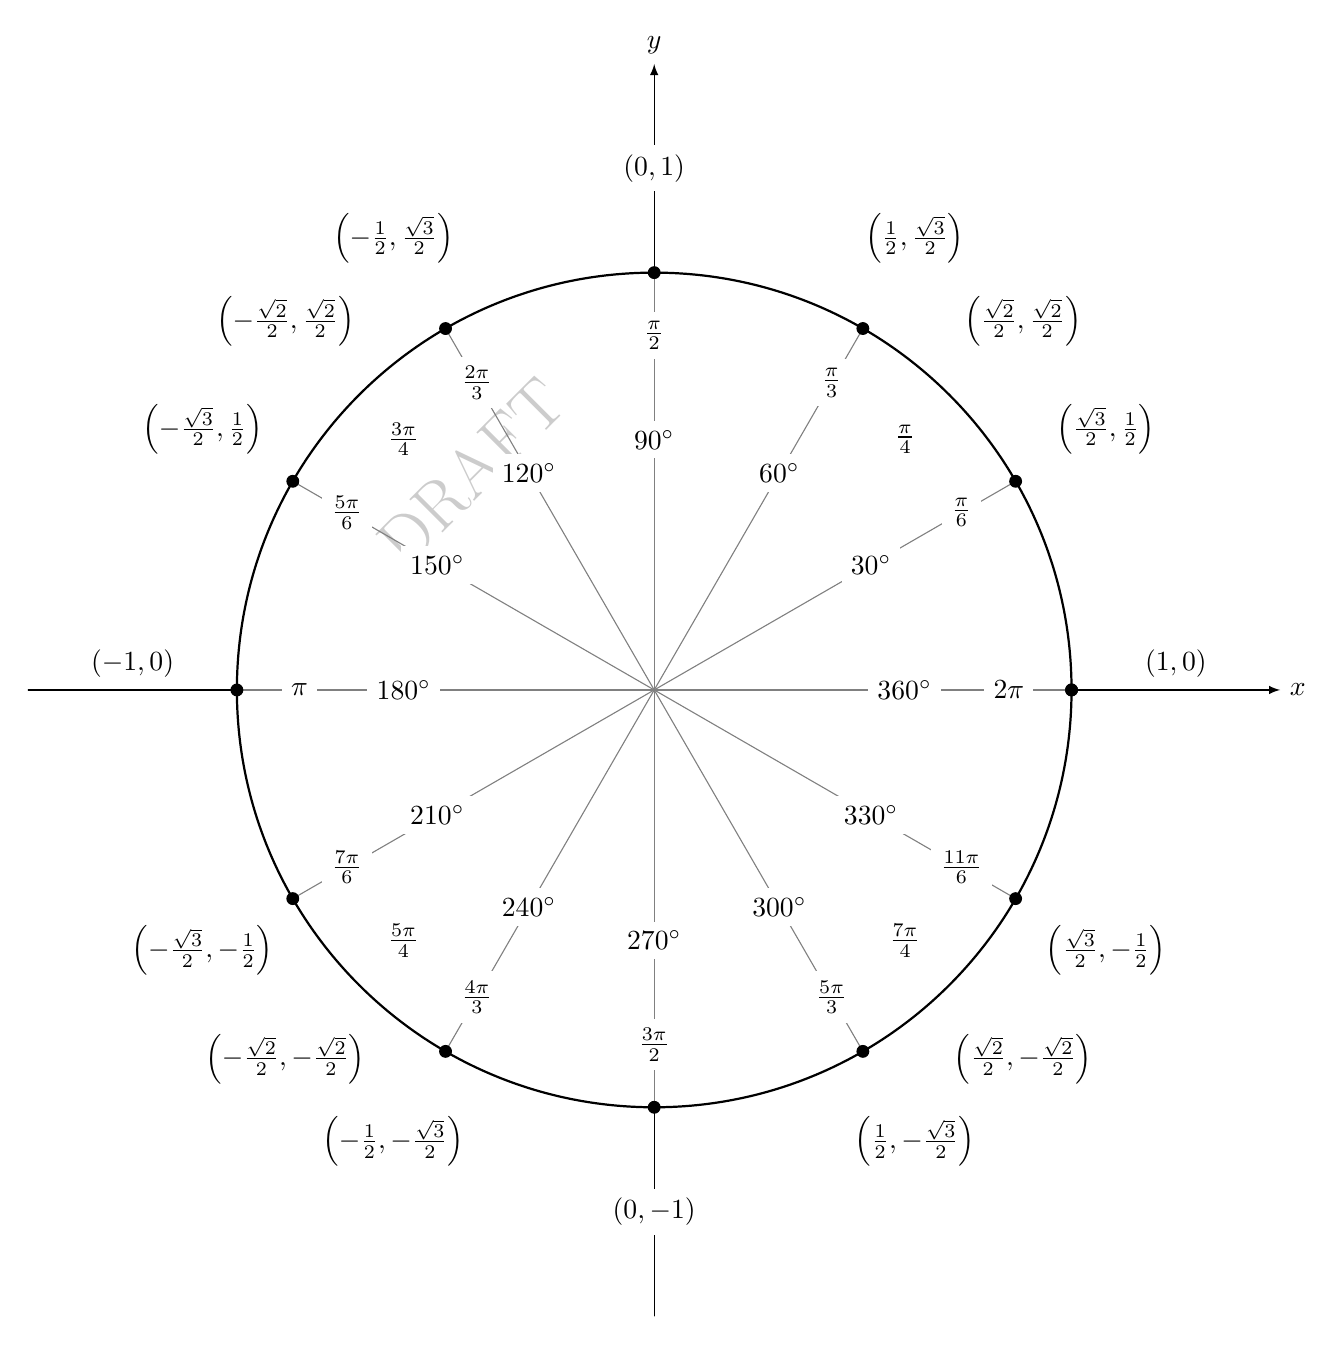
\begin{tikzpicture}[scale=5.3,cap=round,>=latex]
  % draw the coordinates
  \draw[->] (-1.5cm,0cm) -- (1.5cm,0cm) node[right,fill=white] {$x$};
  \draw[->] (0cm,-1.5cm) -- (0cm,1.5cm) node[above,fill=white] {$y$};

  % draw the unit circle
  \draw[thick] (0cm,0cm) circle(1cm);

  \foreach \x in {0,30,...,360} {
    % lines from center to point
    \draw[gray] (0cm,0cm) -- (\x:1cm);
    % dots at each point
    \filldraw[black] (\x:1cm) circle(0.4pt);
    % draw each angle in degrees
    \draw (\x:0.6cm) node[fill=white] {$\x^\circ$};
            
    % 'drop a vertical' as Fran Griffin calls it
    % x-coord = cos(A)
    % y-coord = 0;
%    \draw (\x:0.6cm) -- (\x:0.6cm,0);
  }

    % draw each angle in radians
    \foreach \x/\xtext in {
        30/\frac{\pi}{6},
        45/\frac{\pi}{4},
        60/\frac{\pi}{3},
        90/\frac{\pi}{2},
        120/\frac{2\pi}{3},
        135/\frac{3\pi}{4},
        150/\frac{5\pi}{6},
        180/\pi,
        210/\frac{7\pi}{6},
        225/\frac{5\pi}{4},
        240/\frac{4\pi}{3},
        270/\frac{3\pi}{2},
        300/\frac{5\pi}{3},
        315/\frac{7\pi}{4},
        330/\frac{11\pi}{6},
        360/2\pi}
            \draw (\x:0.85cm) node[fill=white] {$\xtext$};

    \foreach \x/\xtext/\y in {
        % the coordinates for the first quadrant
        30/\frac{\sqrt{3}}{2}/\frac{1}{2},
        45/\frac{\sqrt{2}}{2}/\frac{\sqrt{2}}{2},
        60/\frac{1}{2}/\frac{\sqrt{3}}{2},
        % the coordinates for the second quadrant
        150/-\frac{\sqrt{3}}{2}/\frac{1}{2},
        135/-\frac{\sqrt{2}}{2}/\frac{\sqrt{2}}{2},
        120/-\frac{1}{2}/\frac{\sqrt{3}}{2},
        % the coordinates for the third quadrant
        210/-\frac{\sqrt{3}}{2}/-\frac{1}{2},
        225/-\frac{\sqrt{2}}{2}/-\frac{\sqrt{2}}{2},
        240/-\frac{1}{2}/-\frac{\sqrt{3}}{2},
        % the coordinates for the fourth quadrant
        330/\frac{\sqrt{3}}{2}/-\frac{1}{2},
        315/\frac{\sqrt{2}}{2}/-\frac{\sqrt{2}}{2},
        300/\frac{1}{2}/-\frac{\sqrt{3}}{2}}
            \draw (\x:1.25cm) node[fill=white] {$\left(\xtext,\y\right)$};

    % draw the horizontal and vertical coordinates
    % the placement is better this way
    \draw (-1.25cm,0cm) node[above=1pt] {$(-1,0)$}
          (1.25cm,0cm)  node[above=1pt] {$(1,0)$}
          (0cm,-1.25cm) node[fill=white] {$(0,-1)$}
          (0cm,1.25cm)  node[fill=white] {$(0,1)$};
\end{tikzpicture}
\caption{The Unit Circle, based on work from Supreme Ayal, TiKZ Examples
\cite{HTrCS}}
\end{figure}

A formal definition of the unit circle:
$cos(\theta)$ is the $x$-value of the intersection of the unit circle with the
angle $\theta$.\\
$sin(\theta)$ is the $y$-value of the intersection of the unit circle with the
angle $\theta$\footnote{These words are not quite complete, and would require
the unit circle picture}.

UTUCDTCTV:\footnote{Use the Unit Circle Definition to Calculate The Value}
\begin{align}
  cos(\frac{-2\pi}{3}) & = \ldots
\end{align}
$\pi$ is $\frac{1}{2}$ circle.\\
$\frac{\pi}{3}$ is $\frac{1}{3}$ of $\frac{1}{2}$ a circle.\\
At this point, there has been no trigonometry\ldots \\
% TODO: diagram of above (2pi / 3), drop verticals, & horizontals
The rest of this is high school geometry to determine angles involving
triangles (such as Pythagoras).
% TODO: include pi/3 complement

\subsubsection{Properties of The Unit Circle}
\label{sec:Properties of The Unit Circle}

\begin{align}
  -1 \leq & sin(\theta) \leq & 1 \\
\end{align}
% TODO: 10 O'Clock unit circle
$sin(\theta)$ is the $y$-value on the unit circle which is bound by -1 and 1.

\begin{align}
  sin(-\theta) & = - sin(\theta) \\
\end{align}

% TODO: Picture of right angle triangle
% TODO: Angle sum of a triangle against 2 parallel lines = pi radians 
% TODO: SOH, CAH, TOA
\subsubsection{SOH CAH TOA}
\label{sec:SOHCAHTOA}
\begin{align}
  sin(\theta \ndeg) & = \frac{o}{h} \\
  cos(\theta \ndeg) & = \frac{a}{h} \\
  tan(\theta \ndeg) & = \frac{o}{a}
\end{align}

\subsubsection{Angle Sum Formula}
\label{sec:AngleSumFormula}

There are 3 angle sum formulae to learn, and while the 3rd can be deduced from
the first two, it is easier to just memorise it as the derivation is beyond
the scope of MATH130.

\begin{align}
  sin(\alpha + \beta) & = sin(\alpha)cos(\beta) + cos(\alpha)sin(\beta) \\
  cos(\alpha + \beta) & = cos(\alpha)sin(\beta) - cos(\beta)sin(\alpha) \\
  tan(\alpha + \beta) & = \frac{tan(\alpha) + tan(\beta)}{1 - tan(\alpha)tan(\beta)}
\end{align}

%-----------------------------------------------------------------------------%
%- Algebra :: Polynomials ----------------------------------------------------%
%-----------------------------------------------------------------------------%  
\newpage
\section{TODO: Polynomials}
\label{sec:Polynomials}
\lipsum[1]
%-----------------------------------------------------------------------------%
%- Algebra :: Absolute Values ------------------------------------------------%
%-----------------------------------------------------------------------------%
\newpage
\section{TODO: Absolute Values}
\label{sec:AbsoluteValues}
\lipsum[1]
%-----------------------------------------------------------------------------%
%- Algebra :: Inequalities ---------------------------------------------------%
%-----------------------------------------------------------------------------%
\newpage
\section{TODO: Inequalities}
\label{sec:Inequalities}
\lipsum[1]
%-----------------------------------------------------------------------------%
%- Algebra :: Simultaneous Equations------------------------------------------%
%-----------------------------------------------------------------------------%
\newpage
\section{TODO: Simultaneous Equations}
\label{sec:SimultaneousEquations}
\lipsum[1]
%-----------------------------------------------------------------------------%
%- Algebra :: Matrices -------------------------------------------------------%
%-----------------------------------------------------------------------------%
\newpage
\section{TODO: Matrices}
\label{sec:Matrices}

\begin{align}
  \intertext{Addition}
  \mathbb{Z}_{M,N} & = \mathbb{A} + \mathbb{B} \nonumber \\
         {z}_{i,j} & = {a}_{i,j} + {b}_{i,j} \\
  \intertext{Subtraction}
  \mathbb{Z}_{M,N} & = \mathbb{A} - \mathbb{B} \nonumber \\
         {z}_{i,j} & = {a}_{i,j} - {b}_{i,j} \\
  \intertext{Multiplication}
  \mathbb{Z}_{M,N} & = \mathbb{A} \times \mathbb{B} \nonumber \\
         {z}_{i,j} & = \sum_{k=1}^{N} {a}_{i,k} \times {b}_{k,j}
\end{align}

\subsection{Language of Matrices}
\label{sec:LanguageOfMatrices}

A matrix is nothing more than a bunch of numbers arranged into a grid of
\emph{M} rows and \emph{N} columns and is represented usually by $\mathbb{A}$.
To represent a specific element inside the matrix $\mathbb{A}$, it is usually
referred to as $a_{i,j}$ \footnote{I don't know why we change to lowercase, but
it is the convention. Maybe it is to prevent confusion between referring to a
whole matrix (of particular dimensions) and a specific element of a matrix.}
\\
An example of a ``3 by 4'' matrix called $\mathbb{A}$ is as follows:
\\
\begin{align}
\mathbb{A}_{2,3} & = 
\begin{bmatrix}
  a_{1,1}   &   a_{1,2}   &   a_{1,3}   &   a_{1,4}   \\
  a_{2,1}   &   a_{2,2}   &   a_{2,3}   &   a_{2,4}   \\
  a_{3,1}   &   a_{3,2}   &   a_{3,3}   &   a_{3,4}   \\
\end{bmatrix}
\end{align}
\\
Or more generally:
\\
\begin{align}
\mathbb{A}_{M,N} & = 
\begin{bmatrix}
  a_{1,1}   &   a_{1,2}   &   a_{1,3}   &   \ldots   &   a_{1,j}   \\
  a_{2,1}   &   a_{2,2}   &   a_{2,3}   &   \ldots   &   a_{2,j}   \\
  \vdots    &   \vdots    &   \vdots    &   \ddots   &   \vdots    \\
  a_{i,1}   &   a_{i,2}   &   a_{i,3}   &   \ldots   &   a_{i,j}   \\
\end{bmatrix}
\label{eq:FormOfMatrices}
\end{align}
\\
\emph{In matrix algebra we go vertically describing the rows first then
horizontally we describe the columns.}\footnote{This is in contrast to the
cartesian plane e.g. map reading where we go horizontally then vertically.}

There is also a special kind of matrix called the \emph{identity matrix} often
represented by $\mathbb{I}$. This is a special matrix, which must be square in
shape (ie for $\mathbb{A}_{M,N}, M = N$), and consists of all zeroes except for
a diagonal row of ones from the top left corner to the bottom right corner.

A 4x4 identity matrix:
\begin{align}
  \mathbb{I}_{4,4}~&=
  \begin{bmatrix}
    ~1~&~0~&~0~&~0~\\
    ~0~&~1~&~0~&~0~\\
    ~0~&~0~&~1~&~0~\\
    ~0~&~0~&~0~&~1~\\
  \end{bmatrix}
  \label{eq:4x4IdentityMatrix}
\end{align}

An important property of the identity matrix is that when a matrix is multiplied
by it's identity matrix, the product is the original matrix.
\begin{align}
  \mathbb{A}~\times~\mathbb{I}~&=~\mathbb{A}
\end{align}
Another impotant property is that a matrix can be multiplied by it's identity
matrix in either order (we will see later in section
\ref{sec:MultiplyingMatrices}, Multiplying Matrices that in matrix
algebra, order is important\footnote{as opposed to normal algebra where you can
multiply in any which way and it doesn't matter}.
\begin{align}
  \mathbb{I}~\times~\mathbb{A}~&=~\mathbb{A}
\end{align}

\subsection{Adding Matrices}
\label{sec:AddingMatrices}

Two matrices, $\mathbb{A}$ and $\mathbb{B}$ can be summed if and only if the
matrices have equal rows and columns. To add $\mathbb{A}$ and
$\mathbb{B}$, sum the elements ${a}_{i,j}$ with ${b}_{i,j}$
such that:
\begin{align}
  \mathbb{Z} & = \mathbb{A} + \mathbb{B}
  \intertext{where}
  {z}_{i,j}  & = {a}_{i,j} + {b}_{i,j}
\end{align}
An example:
\begin{align}
  \mathbb{A}_{2,2} & = 
    \begin{bmatrix}
      1  &   5  \\
      3  &  -4  \\
    \end{bmatrix}
  \\
  \mathbb{B}_{2,2} & =
    \begin{bmatrix}
      4  &  -8  \\
      2  &  10  \\
    \end{bmatrix} 
  \\
  \mathbb{A} + \mathbb{B} & =
    \begin{bmatrix}
      1  &   5  \\
      3  &  -4  \\
    \end{bmatrix}
    +
    \begin{bmatrix}
      4  &  -8  \\
      2  &  10  \\
    \end{bmatrix}
  \\
  & =
    \begin{bmatrix}
      (1 + 4)  &  (5 + -8) \\
      (3 + 2)  & (-4 + 10) \\
    \end{bmatrix}
  \\
  & =
    \begin{bmatrix}
      5  & -3 \\
      5  &  6 \\
    \end{bmatrix}
\end{align}

\subsection{Subtracting Matrices}
\label{sec:SubtractingMatrices}
Two matrices, $\mathbb{A}$ and $\mathbb{B}$ can be subtracted if and only if the
matrices have matching rows and columns. To subtract $\mathbb{B}$ from
$\mathbb{A}$, subtract the elements ${b}_{i,j}$ from ${a}_{i,j}$
such that:
\begin{align}
  \mathbb{Z} & = \mathbb{A} - \mathbb{B}
  \intertext{where}
  {z}_{i,j}  & = {a}_{i,j} - {b}_{i,j}
\end{align}
An example:
\begin{align}
  \mathbb{A}_{2,2} & = 
    \begin{bmatrix}
      1  &   5  \\
      3  &  -4  \\
    \end{bmatrix}
  \\
  \mathbb{B}_{2,2} & =
    \begin{bmatrix}
      4  &  -8  \\
      2  &  10  \\
    \end{bmatrix} 
  \\
  \mathbb{A} - \mathbb{B} & =
    \begin{bmatrix}
      1  &   5  \\
      3  &  -4  \\
    \end{bmatrix}
    -
    \begin{bmatrix}
      4  &  -8  \\
      2  &  10  \\
    \end{bmatrix}
  \\
  & =
    \begin{bmatrix}
      (1 - 4)  &  (5 - -8) \\
      (3 - 2)  & (-4 - 10) \\
    \end{bmatrix}
  \\
  & =
    \begin{bmatrix}
      -3  &  13 \\
       1  & -14 \\
    \end{bmatrix}
\end{align}

\subsection{Multiplying Matrices}
\label{sec:MultiplyingMatrices}
Formal definitions for the multiplication of matrices like the one mentioned at
the start of this chapter appear scary, but really, it is just \emph{a lot}\footnote{
Because of this, expect to use up \emph{a lot more} paper.} of simple
additions.

\begin{enumerate}
\item The first rule for multiplying matrices is that the number of columns in
      $\mathbb{A}$ matches the number of rows in $\mathbb{B}$ (that is to say
      $\mathbb{A}_{N}$ = $\mathbb{B}_{M}$).
\item Remember that $\mathbb{Z}_{i,j}$ is a merely sum of several
      multiplication operations.
\end{enumerate}

Formally, $ {z}_{i,j} = \sum_{k=1}^{N} {a}_{i,k} \times {b}_{k,j} $

Broken down, this means for each element in a given row in
$\mathbb{A}$, we must multiply that element by a matching element in it's
corresponding column in $\mathbb{B}$ and sum all the results.

For the matrices $\mathbb{A}$, $\mathbb{B}$ and $\mathbb{P}$:
\begin{align}
\begin{bmatrix}
  ~\textcolor{neekiRed}{p_{1,1}}~&~p_{1,2}~ \\
  ~p_{2,1}~&~\textcolor{neekiGreen}{p_{2,2}}~
\end{bmatrix}
 &~=~ 
\begin{bmatrix}
  ~\textcolor{neekiRed}{a_{1,1}}~&~\textcolor{neekiRed}{a_{1,2}}~&~
                                              \textcolor{neekiRed}{a_{1,3}}~ \\
  ~\textcolor{neekiGreen}{a_{2,1}}~&~\textcolor{neekiGreen}{a_{2,2}}~&~
                                            \textcolor{neekiGreen}{a_{2,3}}~
\end{bmatrix}
~\times~
\begin{bmatrix}
  ~\textcolor{neekiRed}{b_{1,1}}~&~\textcolor{neekiGreen}{b_{1,2}}~ \\
  ~\textcolor{neekiRed}{b_{2,1}}~&~\textcolor{neekiGreen}{b_{2,2}}~ \\
  ~\textcolor{neekiRed}{b_{3,1}}~&~\textcolor{neekiGreen}{b_{3,2}}~
\end{bmatrix}
\intertext{where:}
\textcolor{neekiRed}{p_{1,1}}&\textcolor{neekiRed}{~=~a_{1,1}~\times~b_{1,1}~+~a_{1,2}~\times~b_{2,1}~+~a_{1,3}~\times~b_{3,1}} \nonumber \\
\textcolor{neekiPurple}{p_{2,1}}&~=\textcolor{neekiPurple}{~a_{2,1}~\times~b_{1,1}~+~a_{2,2}~\times~b_{2,1}~+~a_{2,3}~\times~b_{3,1}} \nonumber \\
\textcolor{neekiGreen}{p_{1,2}}&\textcolor{neekiGreen}{~=~a_{1,1}~\times~b_{1,2}~+~a_{1,2}~\times~b_{2,2}~+~a_{1,3}~\times~b_{3,2}} \nonumber \\
p_{2,2}&~=~a_{2,1}~\times~b_{1,2}~+~a_{2,2}~\times~b_{2,2}~+~a_{2,3}~\times~b_{3,2} \nonumber
\end{align}

\subsection{Identity Matrix}
\label{sec:IdentityMatrix}
For the identity matrix:
\begin{align}
  \mathbb{A}~\times~\mathbb{I}~&=~\mathbb{A} \nonumber
\end{align}

Proof by general case:
\begin{align}
  \begin{bmatrix}
    ~1~&~0~\\
    ~0~&~1~\\
  \end{bmatrix}
  \times
  \begin{bmatrix}
    ~a~&~b~\\
    ~c~&~d~\\
  \end{bmatrix}
  &=
  \begin{bmatrix}
    ~[(1~\times~a)+(0~\times~c)]~&~[(1~\times~b)+(0~\times~c)]~\\
    ~[(0~\times~a)+(1~\times~c)]~&~[(0~\times~b)+(1~\times~d)]~\\
  \end{bmatrix}\\
  &=
  \begin{bmatrix}
    ~a~&~b~\\
    ~c~&~d~\\
  \end{bmatrix}
\end{align}

This is the matrix equivalent of the number 1\footnote{NOTE: this is only
equivalent to one, it is not actually the value of one (to my knowledge).}

\begin{align}
  1~\times~a~&=~a \\
  \frac{1}{a}~\times~a~&=~1 \\
  \intertext{in matrix terms:}
  \mathbb{A}^{-1}~\times~\mathbb{A} = \mathbb{I}
\end{align}

This leads into the topic of calculating the inverse of a matrix.

\subsection{Inverse of Matrices}
\label{sec:InverseOfMatrices}
For a 2x2 matrix:
\begin{align}
  \mathbb{A} & = 
    \begin{bmatrix}
      a & b \\
      c & d
    \end{bmatrix}
    \\
  \mathbb{A}^{-1} & =
    \frac{1}{ad-bc} \times
    \begin{bmatrix}
      &~d~&~-b~& \\
      &~-c~&~a~&
    \end{bmatrix}  
\end{align}

For a 3x3 matrix:
%\begin{align}
%
%\end{align}
TODO THIS\ldots

For a 4x4 matrix, in the words of Sal Kahn, ``You'll be there all day, and for a
5x5 you're almost bound to make a mistake and is best left for a
computer.''\footnote{``In my mind, the only thing less pleasant than inverting
a 3 by 3 matrix is inverting a 4 by 4 matrix.'' -- both quotes from
http://www.khanacademy.org/video/inverting-matrices--part-2?playlist=Linear\%20Algebra}

\subsection{TODO: Dividing Matrices}
\label{sec:DividingMatrices}

\subsection{Summary of Matrix Operations}
\label{sec:SummaryOfMatrixOperations}

%-----------------------------------------------------------------------------%
%- Algebra :: Parabolas ------------------------------------------------------%
%-----------------------------------------------------------------------------%
\newpage
\section{Parabolas}
\label{sec:Parabolas}
\begin{figure}[!hbt]
\label{fig:FuncGraphParabola}
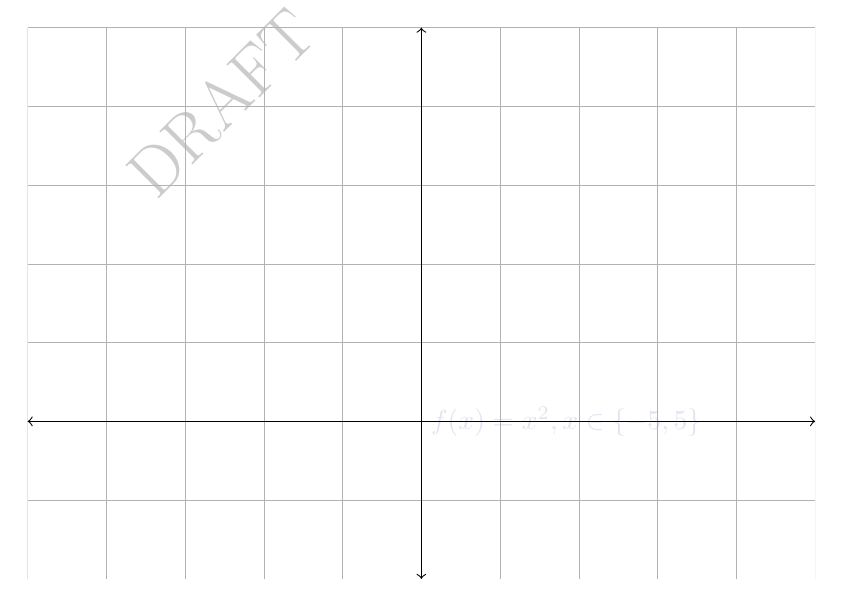
\begin{tikzpicture}[scale=1]
  \def\xmin{-5}
  \def\xmax{5}
  \def\ymin{-2}
  \def\ymax{5}
  \clip
    (\xmin,\ymin) rectangle (\xmax,\ymax);
  \filldraw[fill=blue,fill opacity=0.15, color=neekiBlue, <->, variable=x]
    plot[id=parabola, raw gnuplot, smooth]
    function{
      set xrange [\xmin:\xmax];
      set yrange [\ymin:\ymax];
      plot x**2;}
    node[right] {$f(x) = {x}^{2}, x \in \{ -5,5 \} $};
  % grid
  \draw[very thin, color=black!30, ystep=1, xstep=1]
    (\xmin,\ymin) grid (\xmax,\ymax);
  % x-axis
  \draw[<->]
    (\xmin,0) -- (\xmax,0) node[right] {$x$};
  % y-axis
  \draw[<->]
    (0,\ymin) -- (0,\ymax) node[above] {$f(x)$};
\end{tikzpicture}
\caption{A parabolic function: $f(x) = {x}^{2}$}
\end{figure}
A parabolic function in the form $ f(x) = mx^2 + c$
\begin{table}[!hbt]
\label{tab:PartsOfAParabolicFunction}
\begin{tabularx}{\linewidth}{| l X |}
  \hline
  \multicolumn{2}{|l|}{Where:} \\
  \hline \hline
  m & represents a component of the gradient (covered more in section
  \ref{sec:Differentiation} ``Differentiation''). \\ x & is the independent
  variable\\ y & is the dependent variable\\
\hline
\end{tabularx}
\end{table}
%
%
%-----------------------------------------------------------------------------%
%- Algebra :: Counting -------------------------------------------------------%
%-----------------------------------------------------------------------------%
\newpage
\section{TODO: Counting}
\label{sec:Counting}
%-----------------------------------------------------------------------------%
%- Algebra :: Arithmetic & Geometric Progressions ----------------------------%
%-----------------------------------------------------------------------------%
\newpage
\section{TODO: Arithmetic \& Geometric Progressions}
\label{sec:ArithmeticAndGeometricProgressions}
%
\newpage
\chapter{Calculus}
\label{chap:Calculus}
%-----------------------------------------------------------------------------%
%- Calculus :: Functions & Graphs --------------------------------------------%
%-----------------------------------------------------------------------------%
\section{Functions \& Graphs}
\label{sec:FunctionsAndGraphs}
If you are a computer programmer, the best way to think of a function in maths
is the same way you think of a function in a functional programming language.\\
\\
If you are not a computer programmer, perhaps the best way to think of a
function is like a little machine that takes a number, it does something to
that number, and it displays an output.\footnote{Congratulations, you are now
thinking like a programmer as well as a mathematician!}\\
\\
Here is an example of a function that simply ``doubles'' the input:
\begin{align}
  f(x) & = 2x
  \intertext{Here is what happens when we input the number $5$ into our
  function...}
  f(5)  & = 2(5) \\
        & = 10
  \intertext{And now the number $-5$:}
  f(-5) & = 2(-5) \\
        & = -10
  \intertext{Functions can be (and often are) more complex, here's a
  quadratic function:}
  f(a)  & = {(a+3)}^{2} \\
        & = (a+3)\,(a+3) \\
        & = {a}^{2} + 6a + 9
  \intertext{And if we substitute $5$ in for $a$ we get:}
  f(5)  & = {5}^{2} + 6(5) + 9\\
        & = 25 + 30 + 9 \\
        & = 64
  \intertext{For completeness, if we substitute $-5$ in for $a$ we get:}
  f(-5) & = {-5}^{2} + 6(-5) + 9\\
        & = 25 -6(5) + 9 \\
        & = 4
\end{align}
When it comes to graphing functions, you can rename your $y$ axis to equal
$f(x)$, so graphing your function is now the same as before graphs with one
additional bonus: now you can let $x$ be an abitrary number\footnote{This is
called a \emph{independent variable}} as part of the function. Figure
\ref{fig:FuncGraphLinear} shows a function, $f(x) = {x}$.\\
Types of graphs that can be encountered in MATH130:\\
\begin{enumerate}
  \item Line \ref{fig:FuncGraphLinear}
  \item Parabola \ref{fig:FuncGraphParabola}
  \item Hyperbola \ref{fig:FuncGraphHyperbola}
  \item Cubic \ref{fig:FuncGraphCubic}
  \item Absolute \ref{fig:FuncGraphAbsolute}
\end{enumerate}

A function has a \emph{domain} which is all the acceptable values of $x$ as
inputs that the function can use. Some examples:

\begin{align}
   f(x) & = x^{2} \nonumber \\
   domain: { 0 \leq x \geq 0 } \\
   \\
   f(x) & = \frac{1}{x} \nonumber \\
   domain: { x \neq 0 } \\
   \\
   f(x) & = \sqrt{x} \nonumber \\
   domain: { x \geq 0 } \\
   \\
   f(x) & = \sqrt{x-2} + \sqrt{5 + x} \nonumber \\
   domain: (x-2) & \geq 0 \\
      \therefore & \geq 2 \\
      \and \\
   domain: 5 + x & \geq 0 \\
      \therefore & \geq -5 \\
   and so:\\
   {x: x \geq 2}
\end{align}
The last equation demonstrates that the domain is the more restrictive of
the conditions of the two ``sub-domains'' of each square root portion of the
function.

\subsection{Arithmetic With Functions}
\label{sec:ArithmeticWithFunctions}

Suppose we have:
\begin{align}
  f(x) & = x^{2} + 1 \\
  g(x) & = \frac{1}{1-x} \\
  \intertext{and}
  h    & = f(x) + g(x) \\
  \intertext{then}
       & = x^{2} + 1 + \frac{1}{1-x} \\
  \intertext{however, if}
  i    & = f(x) \times g(x) \\
  \intertext{then}
       & = (x^{2} + 1) \times (\frac{1}{1-x}) \\
  \intertext{however, if}
  j    & = f \circ g \\
  \intertext{then}
       & = j(x) = f(g(x)) \\
       & = (\frac{1}{1-x})^{2} + 1
\end{align}
\quote{``Remember to ``algebra'' the function to
minimise them and to see if they equal a simpler equation''}\footnote{according to Gareth Richardson}

%
\clearpage
\subsection{Linear Functions}
\label{sec:LinearFunctions}
\begin{figure}[!hbt]
\label{fig:FuncGraphLinear}
\begin{tikzpicture}[scale=0.5]
  \label{fig:FuncGraphLine}
  \draw[<->]  (-3.9, -1.9) -- (3.9,9.9) node[right] {$f(x) = mx + b$};
  \draw[<->]   (0.0, -1.9) -- (0.0,9.9) node[above] {$f(x)$};
  \draw[<->]  (-3.9,  0.0) -- (3.9,0.0) node[right] {$x$};
\end{tikzpicture}
\caption{A linear function: $f(x) = mx + b$}
\end{figure}
%
Linear function in the \emph{General Form} $Ax + By + C= 0$. It may also take
the handy \emph{Slope-intercept form} $ f(x) = mx + b $. This is useful because
the gradient of the line cane be read straight from the equation, and is just
a rearrangement of the general form. 
\begin{table}[!hbt]
\label{tab:PartsOfALinearFunction}
\begin{tabularx}{\linewidth}{| l X |}
  \hline
  \multicolumn{2}{|l|}{Where:} \\
  \hline \hline
  m & represents the gradient\\
  x & is the independent variable\\
  y & is the dependent variable\\
\hline
\end{tabularx}
\end{table}

If given only 2 points and we are to find the equation of the line:
\begin{enumerate}
  \item we need to determine the gradient
  \item we need to substitute the x,y values in to form the equation
\end{enumerate}

Determining the gradient is done using the formula:
\begin{align}
  \frac{y_{2} - y_{1}}{x_{2} - x_{1}} & = m
\end{align}

Example: we are given the points (7,1), (2,5) and need to find the equation of
the line connecting these points.
\begin{align}
  \frac{5 - 1}{2 - 7} & = \frac{4}{-5}\\
    & = -\frac{4}{-5}
\end{align}

If we want to find a parallel line passing through specific points, remember
that the gradient ($m$) must be the same in both equations, and we must
subtitute the $x$ and $y$ values for the specific points into the new arbitrary
equation to solve for the new equation:

Example: find an equation for the line through $(3,4)$ and parallel to the line
through $(7,1)$ and $(2,5)$ from out previous example:
\begin{align}
  \intertext{let}
  m & = -\frac{4}{5} \nonumber \\
  \intertext{substitute x,y values into slope-intercept equation}
  y & = mx + b \nonumber \\
  4 & = -frac{4}{5}\times3 + b
  \intertext{and solve for b}
  4 + \frac{4}{5}\times3 & = b \\ 
  4 + \frac{12}{5}       & = b \\
  \frac{32}{5}           & = b \\
  \therefore y & = -\frac{4}{5}x + \frac{32}{5}
\end{align}
%
\clearpage
\subsection{Parabolic Functions}
\label{sec:ParabolicFunctions}
For an introduction to parabolas, it is highly recommended to read section
\ref{sec:Parabolas}, ``Parabolas''.
\clearpage
\subsection{Hyperbolic Functions}
\begin{figure}[!htb]
\label{fig:FuncGraphHyperbola}
\begin{tikzpicture}[samples=50,scale=1]
   \draw[color=neekiRed,domain=-5:-0.2,variable=x]
     plot[id=hyperbx.neg] function{1/x}
     node[right] {$f(x) = \frac{1}{x}, x \in \{ -5,-\frac{1}{5} \} $};
   \draw[color=neekiBlue,domain=0.2:5,variable=x]
   plot[id=hyperbx.pos] function{1/x}
     node[right] {$f(x) = \frac{1}{x}, x \in \{ \frac{1}{5},5 \} $};
  \draw[<->]  (0.0,-5.0) -- (0.0,5.0) node[above] {$f(x)$};
  \draw[<->] (-5.0, 0.0) -- (5.0,0.0) node[right] {$x$};
\end{tikzpicture}
\caption{A hyperbolic function: $f(x) = \frac{1}{x}$}
\end{figure}
A hyperbolic function in the form $ f(x) = \frac{1}{x}$
\begin{table}[!hbt]
\label{tab:PartsOfAHyperbolicFunction}
\begin{tabularx}{\linewidth}{| l X |}
  \hline
  \multicolumn{2}{|l|}{Where:} \\
  \hline \hline
  x & is the independent variable\\
  y & is the dependent variable\\
\hline
\end{tabularx}
\end{table}
%
\clearpage
\subsection{Cubic Functions}
\begin{figure}[!hbt]
\label{fig:FuncGraphCubic}
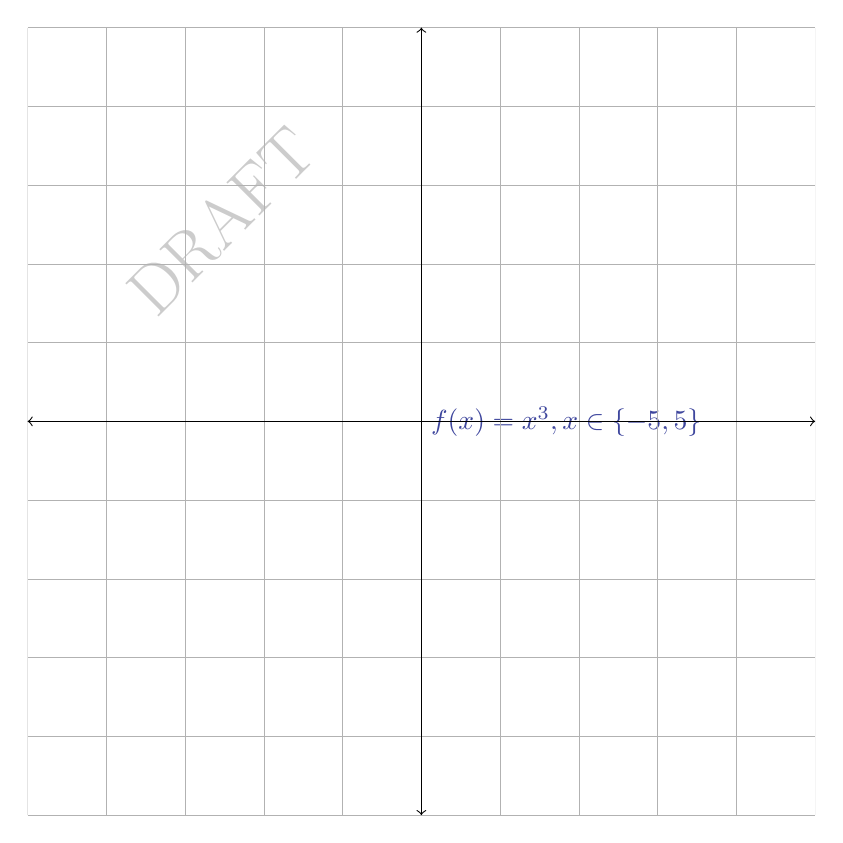
\begin{tikzpicture}[scale=1]
  \def\xmin{-5}
  \def\xmax{5}
  \def\ymin{-5}
  \def\ymax{5}
  \clip
    (\xmin,\ymin) rectangle (\xmax,\ymax);
  \draw[color=neekiBlue, <->, variable=x]
    plot[id=parabola, raw gnuplot, smooth]
    function{
      set xrange [\xmin:\xmax];
      set yrange [\ymin:\ymax];
      plot x**3;}
    node[right] {$f(x) = {x}^{3}, x \in \{ -5,5 \} $};
  % grid
  \draw[very thin, color=black!30, ystep=1, xstep=1]
    (\xmin,\ymin) grid (\xmax,\ymax);
  % x-axis
  \draw[<->]
    (\xmin,0) -- (\xmax,0) node[right] {$x$};
  % y-axis
  \draw[<->]
    (0,\ymin) -- (0,\ymax) node[above] {$f(x)$};
\end{tikzpicture}
\caption{A cubic function: $f(x) = {x}^{3}$}
\end{figure}
A cubic function in the form $ f(x) = mx^3 + c$
\begin{table}[!hbt]
\label{tab:PartsOfACubicFunction}
\begin{tabularx}{\linewidth}{| l X |}
  \hline
  \multicolumn{2}{|l|}{Where:} \\
  \hline \hline
  m & represents a component of the gradient (covered more in section
  \ref{sec:Differentiation} ``Differentiation''). \\ x & is the independent
  variable\\ y & is the dependent variable\\
  x & is the independent variable\\
  y & is the dependent variable\\
\hline
\end{tabularx}
\end{table}
%
\clearpage
\subsection{Absolute Value Functions}
\begin{figure}[!hbt]
\label{fig:FuncGraphAbsolute}
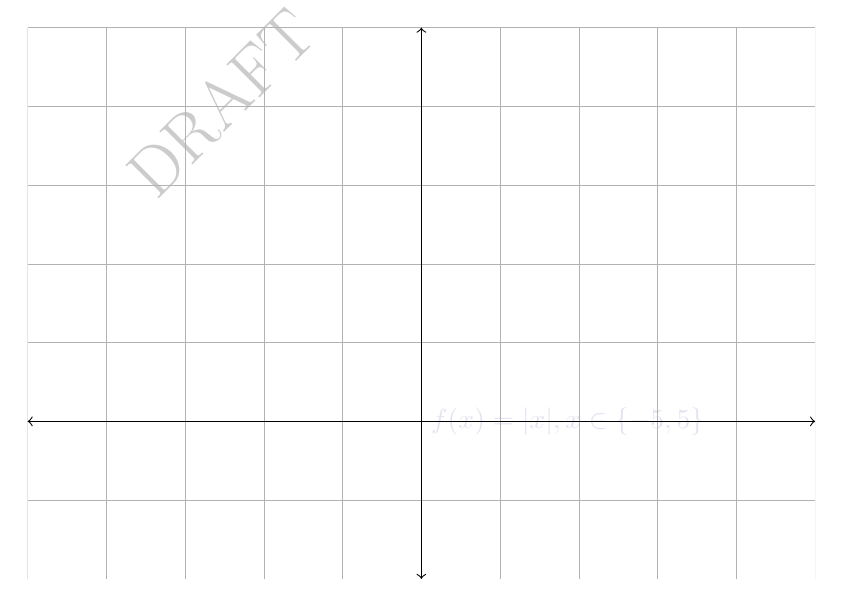
\begin{tikzpicture}[scale=1]
 \def\xmin{-5}
 \def\xmax{5}
 \def\ymin{-2}
 \def\ymax{5}
 \clip
   (\xmin,\ymin) rectangle (\xmax,\ymax);
 \filldraw[fill=blue,fill opacity=0.15, color=neekiBlue, <->, variable=x]
   plot[id=parabola, raw gnuplot, smooth]
   function{
     set xrange [\xmin:\xmax];
     set yrange [\ymin:\ymax];
     plot abs(x);}
   node[right] {$f(x) = |x|, x \in \{ -5,5 \} $};
 % grid
 \draw[very thin, color=black!30, ystep=1, xstep=1]
   (\xmin,\ymin) grid (\xmax,\ymax);
 % x-axis
 \draw[<->]
   (\xmin,0) -- (\xmax,0) node[right] {$x$};
 % y-axis
 \draw[<->]
   (0,\ymin) -- (0,\ymax) node[above] {$f(x)$};
\end{tikzpicture}
\caption{A function of absolute value: $f(x) = |x|$}
\end{figure}
An absolute function in the form $ f(x) = |x|$
\begin{table}[!hbt]
\label{tab:PartsOfAnAbsoluteFunction}
\begin{tabularx}{\linewidth}{| l X |}
  \hline
  \multicolumn{2}{|l|}{Where:} \\
  \hline \hline
  m & represents a component of the gradient (covered more in section
  \ref{sec:Differentiation} ``Differentiation''). \\ x & is the independent
  variable\\ y & is the dependent variable\\
  x & is the independent variable\\
  y & is the dependent variable\\
\hline
\end{tabularx}
\end{table}
\clearpage
%
%-----------------------------------------------------------------------------%
%- Calculus :: Lines & Limits ------------------------------------------------%
%-----------------------------------------------------------------------------%
\newpage
\section{Limits}
\label{sec:Limits}
There are some types of functions you may be asked to evaluate for various
values of $x$ which are unreasonable. One such example is the hyperbolic
function $f(x) = \frac{1}{x} $ where $x = 0$. In MATH130, we consider this value
an illegal or ``undefined'' value - but there is still a way to evaluate it.
Consider taking a table of values\ref{tab:LimitsHyperbolaExample}:
\begin{table}[!hbt]
\label{tab:LimitsHyperbolaExample}
\begin{tabularx}{\textwidth}{| c || r | r | r | r | r | r | r | r | r | r | X |}
  \hline
  x & 5    & 4    & 3    & 2    & 1    & 0.8  & 0.6  & 0.4  & 0.2  & 0.1 & \ldots \\
  \hline
  y & 0.20 & 0.25 & 0.33 & 0.50 & 1.00 & 1.25 & 1.67 & 2.50 & 5.00 & 10.00 &
  \ldots \\
  \hline
\hline
\end{tabularx}
\caption{Table of values for hyperbolic function $f(x) = \frac{1}{x}$}
\end{table}
Note how as $x$ gets smaller, $y$ gets bigger. The way this is formally worded
is ``as $x$ approaches $0$, $y$ approaches infinity, and written:
\begin{align}
  x \to 0 & \; f(x) \to \infty
\end{align}
From this point, we can see that $x$ cannot be zero, however all other
$\mathbb{R}$ are acceptable. Building on this we can define it as a set:
\begin{align}
  & x \to 0 \; f(x) \to \infty \nonumber \\
  & x \in \{ \mathbb{R}, x \neq 0 \}
\end{align}
The key to understanding how limits work is to identify what $x$ values are
undefined or otherwise illegal. Key indicators of this phenomena are when you
see $x$ inside a squareroot sign, or as a divisor in a quotient: 
%-----------------------------------------------------------------------------%
%- Calculus :: Differentiation -----------------------------------------------%
%-----------------------------------------------------------------------------%
\newpage
\section{Differentiation}
\label{sec:Differentiation}
In overly simplified terms, differentiation is the process of taking a curve
on a graph and finding what the gradient of that curve is. There are 4
methods which are useful for MATH130. These are:
\begin{itemize}
  \item Power Method (well, that's what I call it)
  \item Product Rule
  \item Quotient Rule
  \item Chain Rule
\end{itemize}
Because the notion of calculus was a joint effort between several
mathematicians \footnote{Gottfried Leibniz woke up one day and thought ``I'm
going to invent a whole new branch of mathematics to annoy students for the
next few hundred years.'' Approximately 10 years earlier, Sir Isaac Newton
thought ``I know what will really get Leibniz's goat... I'll get the drop on
him with this idea I have.'' Consequently, the two never became friends.}
operating in secret, and without a project manager there are two important
notations.\footnote{there are more, but we don't need to know about them for
MATH130}\\
\\
The first notation is the ``dash'', ``prime'', or ``Lagrange's'' notation and
appears as such:
\begin{align}
   f(x) & = ... \\
  f'(x) & = ...
  \intertext{Secondly is Leibniz's notation:}
   f(x)\derivative &= ...
  \intertext{Euler's notation: (not so common in MATH130)}
   Df(x) & = ... \\
\end{align}
Each notation has their merits and usefulness; Lagrange's form is neat and
compact for simple derivatives, however Leibniz's notation describe what is
being differentiated and what is in respect to, which is useful for the chain
rule discussed shortly. As such, it is important to be familiar with all the
above forms as they will often be used interchangeably for brevity,
neatness and ease of memorising them. In terms of how you answer a question - 
if there is no stated style of notation, go for what ``looks'' like it works
\footnote{Munner's Law: If it looks wrong it probably is. -- Cliff Munro,
1996 Cranbrook School, Design and Technology teacher. Author's corollary: If it
doesn't look wrong, hopefully it's right.} and is clear and neat. Clear and
neat usually results in the marker understanding what you are on about, so even
if you are wrong, you might get partial marks.\\
\\
A useful tip, when you are first getting used to differentiation, it may be
handy to use Leibniz's notation and say in your mind what you are
differentiating, and what it is in respect to.
%-----------------------------------------------------------------------------%
%- Calculus :: Differentiation :: Power Method -------------------------------%
%-----------------------------------------------------------------------------%
\newpage
\subsection{Power Method}
\label{sec:PowerMethod}
The power method is by far the easiest to understand of all 3 methods, and if
possible, it may be easier to rearrange a part of an equation into index
notation and differentiate that way. This method is not always possible,
but by using the power laws from the series of equations starting with
\ref{eq:ExponentLaw_Power0}, sometimes a shortcut can be made, which is why
Section \ref{sec:ExponentialsAndLogarithms} important to know very well.\\
\\
Put simply, the power method can be understood as ``multiply the base by the
power and subtract one from the power'', and is demonstrated in equation
\ref{eq:DiffPowerMethod} below.
\begin{align}
  f(x) & =   {x}^{a} + k \label{eq:DiffPowerMethodKValue} \\
  f(x)\derivative & =   a{x}^{a-1} \label{eq:DiffPowerMethod}
\end{align}
The value $k$ represents a constant, often just a plain number, though it
doesn't have to be. The important thing about the $k$-value in this example is
that there is no $x$ component. Hence it ``disappears''.\\
Functions may have more than one term, consider the following quadratic:
\begin{align}
  f(x)            & = {x}^{2} + 2xb + {b}^{2} \\
  f(x)\derivative & = 2{x}^{1} + 2b \\
                  & = 2(x+b) \label{eq:DiffPowerMethodRespectTo}
\end{align}
Here we are asked to differentiate with respect to $x$ (denoted by the symbol
$\derivative$). To do this, we bring the power of ${x}^{2}$ to the front, and
subtract 1 to give $2{x}^{1}$, and we do the same for the term ${2xb}$ by
looking at the invisible power (it's there, we just don't write it out of
laziness!\footnote{Or convenience, neatness, brevity.}): $2*{x}^{1}*b$
%-----------------------------------------------------------------------------%
%- Calculus :: Differentiation :: Product Rules ------------------------------%
%-----------------------------------------------------------------------------%
\newpage
\subsection{Product Rule}
\label{sec:ProductRule}
A function $f(x)$ is a product of two functions, $u(x) * v(x)$. For example:
\begin{align}
  f(x) & = {x}^{3} sin(x) \label{eq:DiffProdEx1}\\
       & = u(x)v(x)
\end{align}
In this case, we can clearly see that $u(x)$ could be ${x}^{3}$ and $v(x)$
could be $sin(x)$. While there is a mathematical proof\footnote{refer to section
\ref{eq:ProofOfProductRule} of appendix} it is not necessary for MATH130.
All we need to know is:
\begin{align}
             f(x) & = u(x)v(x) \\
  f(x)\derivative & = u(x)\,v(x)\derivative + u(x)\derivative\,v(x) \\
            f'(x) & = u(x)\,v'(x) + u'(x)\,v(x)
\end{align}
So for \ref{eq:DiffProdEx1}, to find the derivative:
\begin{align}
            f(x)  & = {x}^{3}\,sin(x) \nonumber \\
  f(x)\derivative & = {x}^{3}\,sin(x)\derivative + {x}^{3}\derivative\,sin(x) \\
                  & = {x}^{3}\,cos(x) + 3{x}^{2}\,sin(x) \\
  \therefore {x}^{3}\,sin(x)\derivative  & = {x}^{3}\,cos(x) + 3{x}^{2}\,sin(x)
\end{align}
%-----------------------------------------------------------------------------%
%- Calculus :: Differentiation :: Quotient Rule ------------------------------%
%-----------------------------------------------------------------------------%
\newpage
\subsection{Quotient Rule}
\label{sec:QuotientRule}
A quotient is a division - just like from primary school: $\frac{u}{v}$.
Previously we may have called the $u$ part the numerator, nowadays it is
called the \emph{dividend}, and the $v$ denominator previously called the
denominator is now called the \emph{divisor}, with the \emph{quotient} being
the result.\\
\\
To do quotient rule differentiation, we are actually using a modified version
of the product rule, however for MATH130 it is only required to think of it as a
separate rule.\footnote{Mathematical proof of this is in section 
\ref{eq:ProofOfQuotientRule} of the appendix.} The rule takes the form of:
\begin{align}
  f(x) & = \frac{u}{v} \\
  f(x)\derivative & = \frac{u\derivative\,v - u\,v\derivative}{{v}^{2}}
                      \label{eq:DiffQuot1}
  \intertext{ Although both \ref{eq:DiffQuot1} and \ref{eq:DiffQuot2} are
  identical, \ref{eq:DiffQuot2} is tidier, and may be easier to remember.}
  f'(x) & = \frac{u'\,v - u\,v'}{{v}^{2}} \label{eq:DiffQuot2}
\end{align}
Consider the following example:
\begin{align}
  f(x)  & = \frac{{x}^{2}}{4x} \\
  f'(x) & = (4x){x}^{2}\derivative - {x}^{2} (4x\derivative) \\
  f'(x) & = (4x)2x - {x}^{2}\,(4) \\
  f'(x) & = 8{x}^{2} - 4{x}^{2} \\
  f'(x) & = 4{x}^{2}
\end{align}
%-----------------------------------------------------------------------------%
%- Calculus :: Differentiation :: Chain Rule ---------------------------------%
%-----------------------------------------------------------------------------%
\newpage
\subsection{Chain Rule}
\label{sec:ChainRule}
The chain rule is useful for differentiation a function $f(x)$ where there are
functions inside of functions (such as $ln(sin(x))$). To do this, we break
the function up into it's components, give them some names \footnote{''
\emph{Let}`` is possibly the most important word you will come across in
mathematics. You can use it to redefine stuff if it's too complex and break it
into smaller manageable pieces and put it back together again." -- Chris
Gordon, MATH130 lecturer, Macquarie University, 2011} and apply the chain rule.
The rule takes the form as follows:
\begin{align}
  f(x) & = v(u(x)) \\
  f(x)\derivative & = f\derivative[u]\,u\derivative[x] \label{eq:DiffChainRule}
\end{align}
Here is an example of where we might use the chain rule:\footnote{Note that the
$v$ function above in this example is simply ${u}^{3}$.}\footnote{While we
could use the power method to solve this particular problem in 2 steps, we will
demonstrate chain rule first, and then the power method.}
\begin{align}
  f(x) & = {({x}^{2})}^{3}
  \intertext{Let $u = {x}^{2}$ such that}
  f(x) & = {u}^{3} \label{eq:DiffChainRuleLet}
  \intertext{The first step in \ref{eq:DiffChainRuleLet} is to identify the
  chain rule, and to name the function inside $u$. It just makes things
  easier this way for most of the time.}
  f(x)\derivative & = f\derivative[u] * u\derivative[x] \\
                  & = \left[ 3{u}^{2} \right]\,\left[ 2x \right]
  \intertext{\ref{eq:DiffChainRuleLet} It often helps to rewrite the equation
  in terms of $f(x)$ and $u$, and then to write out the chain rule. Normally we
  are differentiating $f(x)$ with respect to $x$ ($\derivative$). Here we
  differentiate $f(x)$ with respect to $u$ (ie $\derivative[u]$) \emph{THEN}
  multiply by $u$. The rest is plain old algebra. So.. substitue values back
  for $u$.}
                  & = \left[ 3{({x}^{2})}^{2} \right] * 2x
  \intertext{simplify the first set of brackets with basic power laws}
                  & = (3{x}^{4})(2x) \\
                  & = 6{x}^{5}
\end{align}
As a point of exercise, here's how much faster it is using the power method:
\begin{align}
  f(x) & = {({x}^{2})}^{3} \\
  f(x)  & = {x}^{6}
  \intertext{Now we use the differentiation power method, bring the power out
  the front and reduce the power by one}
  f(x)\derivative & = 6{x}^{5}
  \intertext{Look! Only two steps!}
\end{align}
It should be noted however, that power method cannot be used for all chain rule
problems (in fact, most of the time it can't - but for easy ones like this, it
is far more efficient to use power method.) The following example cannot use
power method, and we \emph{should} use the chain rule:
\begin{align}
  f(x) & = ln(sin(x)) \\
  \intertext{Let } u(x) & = sin(x)
\end{align}
%-----------------------------------------------------------------------------%
%- Calculus :: Practical Uses of Differentiation -----------------------------%
%-----------------------------------------------------------------------------%
\newpage
\section{TODO: Practical uses of Differentiation}
\label{sec:PracticalUsesOfDifferentiation}
\lipsum[1]
%-----------------------------------------------------------------------------%
%- Calculus :: Differentiation of Exponents and Logs -------------------------%
%-----------------------------------------------------------------------------%
\newpage
\section{TODO: Differentiation of Exponents and Logs}
\label{sec:DifferentiationOfExponentsAndLogs}
\lipsum[1]
%-----------------------------------------------------------------------------%
%- Calculus :: Differentiation of Trigonometric Functions --------------------%
%-----------------------------------------------------------------------------%
\newpage
\section{Differentiation of Trigonometric Functions}
\label{sec:DifferentiationOfTrigFunctions}
Consider the plot of the function $f(x) = sinx$
\begin{figure}[!htb]
\label{fig:GraphTemplate}
\begin{tikzpicture}[samples=50,scale=1]
   \draw[color=neekiRed,domain=0:pi,variable=x]
     plot[id=sinx] function{1/x}
     node[right] {$f(x) = \frac{1}{x}, x \in \{ -5,-\frac{1}{5} \} $};
%   \draw[color=neekiBlue,domain=0:5,variable=x]
  \draw[<->]  (0.0,-5.0) -- (0.0,5.0) node[above] {$f(x)$};
  \draw[<->] (-5.0, 0.0) -- (5.0,0.0) node[right] {$x$};
\end{tikzpicture}
\caption{A hyperbolic function: $f(x) = \frac{1}{x}$}
\end{figure}
A hyperbolic function in the form $ f(x) = \frac{1}{x}$
\begin{table}[!hbt]
\label{tab:GraphTemplateParts}
\begin{tabularx}{\linewidth}{| l X |}
  \hline
  \multicolumn{2}{|l|}{Where:} \\
  \hline \hline
  x & is the independent variable\\
  y & is the dependent variable\\
\hline
\end{tabularx}
\end{table}
%
Here are some equations that are handy to remember. Source \cite{RHBDiffQuickStart}.
\begin{align}
  {x}^{n}\derivative & = n{x}^{n-1} \\
  {\emph{e}}^{ax}\derivative & = a{\emph{e}}^{ax} \\
  ln(ax)\derivative & = \frac{1}{x} \\
  sin(ax)\derivative & = (a)cos(ax) \\
  cos(ax)\derivative & = (-a)sin(ax) \\
  tan(ax)\derivative & = (a){sec}^{2}(ax) \\
  sec(ax)\derivative & = (a)sec(ax)tan(ax) \\
  csc(ax)\derivative & = (-a)csc(ax)cot(ax) \\
  cot(ax)\derivative & = (-a){csc}^{2}(ax) \\
  {sin}^{-1}(\frac{x}{a})\derivative & = \frac{1}{\sqrt[2]{{a}^{2} - {x}^{2}}} \\
  {sin}^{-1}(\frac{x}{a})\derivative & = \frac{-1}{\sqrt[2]{{a}^{2} - {x}^{2}}} \\
  {sin}^{-1}(\frac{x}{a})\derivative & = \frac{a}{\sqrt[2]{{a}^{2} - {x}^{2}}}  
\end{align}
For a proof, refer to appendix section \ref{sec:DiffTrigProof},
``Differentiation of Trig Functions Proof''
%-----------------------------------------------------------------------------%
%- Calculus :: Differentiation of Trigonometric Functions --------------------%
%-----------------------------------------------------------------------------%
\newpage
\section{TODO: Maxima and Minima}
\label{sec:MaximaAndMinima}
\lipsum[1]
%-----------------------------------------------------------------------------%
%- Calculus :: Differentiation of Trigonometric Functions --------------------%
%-----------------------------------------------------------------------------%
\newpage
\section{TODO: Grokking Word Problems}
\label{sec:GrokkingWordProblems}
\lipsum[1]
%-----------------------------------------------------------------------------%
%- Calculus :: Differentiation of Trigonometric Functions --------------------%
%-----------------------------------------------------------------------------%
\newpage
\section{TODO: Curve Sketching}
\label{sec:CurveSketching}
\lipsum[1]
%-----------------------------------------------------------------------------%
%- Calculus :: Differentiation of Trigonometric Functions --------------------%
%-----------------------------------------------------------------------------%
\newpage
\section{TODO: Integration}
\label{sec:Integration}
tl;dr: Integration is the reverse process of Differentiation.
%-----------------------------------------------------------------------------%
%- Calculus :: Differentiation of Trigonometric Functions --------------------%
%-----------------------------------------------------------------------------%
\newpage
\section{TODO: Newton's Method}
\label{sec:NewtonsMethod}
\lipsum[1]
%-----------------------------------------------------------------------------%
%- Calculus :: Differentiation of Trigonometric Functions --------------------%
%-----------------------------------------------------------------------------%
\newpage
\section{TODO: Integration: The 2 Types}
\label{sec:IntegrationThe2Types}
Outline anti-derivatives (ie indefinite integrals) and definite integrals.
%-----------------------------------------------------------------------------%
%- Calculus :: Differentiation of Trigonometric Functions --------------------%
%-----------------------------------------------------------------------------%
\newpage
\section{TODO: Practical uses of Integration}
\label{sec:PracticalUsesOfIntegration}
\lipsum[1]
%-----------------------------------------------------------------------------%
%- Calculus :: Differentiation of Trigonometric Functions --------------------%
%-----------------------------------------------------------------------------%
\newpage
\section{TODO: Average values of a function}
\label{sec:AverageValuesOfAFunction}
\lipsum[1]
%-----------------------------------------------------------------------------%
%- Calculus :: Differentiation of Trigonometric Functions --------------------%
%-----------------------------------------------------------------------------%
\newpage
\section{TODO: Trapezoidal Rule}
\label{sec:TrapezoidalRule}
\lipsum[1]
%-----------------------------------------------------------------------------%
%- Calculus :: Differentiation of Trigonometric Functions --------------------%
%-----------------------------------------------------------------------------%
\newpage
\section{TODO: Simpson's Rule}
\label{sec:SimpsonsRule}
\lipsum[1]
%-----------------------------------------------------------------------------%
%- Appendix ------------------------------------------------------------------%
%-----------------------------------------------------------------------------%
\newpage
\chapter{Appendix}
\label{chap:Appendix}
\section{Algebra}
\lipsum[1]
\section{Calculus}
\label{sec:AppCalculus}
%
%-----------------------------------------------------------------------------%
%- Appendix :: Proof of Product Rule -----------------------------------------%
%-----------------------------------------------------------------------------%
\newpage
\subsection{Proof of Product Rule}
\label{sec:ProofOfProductRule}
\begin{align} 
  \label{eq:ProofOfProductRule}
  x & = 1
\end{align}
%-----------------------------------------------------------------------------%
%- Appendix :: Proof of Quotient Rule ----------------------------------------%
%-----------------------------------------------------------------------------%
\newpage
\subsection{Proof of Quotient Rule}
\label{sec:ProofOfQuotientRule}
\begin{align}
  \label{eq:ProofOfQuotientRule}
  x & = 1
\end{align}
%-----------------------------------------------------------------------------%
%- Appendix :: Proof of Chain Rule -------------------------------------------%
%-----------------------------------------------------------------------------%
\newpage
\subsection{Proof of Chain Rule}
\label{sec:ProofOfChainRule}
\begin{align}
  \label{eq:ProofOfChainRule}
  x & = 1
\end{align}
%-----------------------------------------------------------------------------%
%- Appendix :: Differentiation Quickstart ------------------------------------%
%-----------------------------------------------------------------------------%
\newpage
\subsection{Differentiation of Trig Functions Proof}
\label{sec:DiffTrigProof}
If we have the function $f(x) = sinx$, and take two points, $P$ and $Q$ where
$P = (x,f(x))$ and $Q = (x+h, f(x+h)$ where $h \neq 0$ we can construct a line
joining $P$ and $Q$, and the gradient of this line is given by the ``rise
over run'' formula:
\begin{align}
  \frac{\Delta Y}{\Delta X} & = \frac{f(x+h) - f(x)}{(x+h) - x} \\
                            & = \frac{sin(x+h) - sinx}{h}
\end{align}
%-----------------------------------------------------------------------------%
%- Acknowledgment ------------------------------------------------------------%
%-----------------------------------------------------------------------------%
\newpage
\section{Acknowledgements}
\label{sec:Acknowledgements}
I (Adam) found this to be a particularly big project for me, with a huge
learning curve whilst trying to learn \LaTeX to author this document, whilst
making sure I got as much of the MATH130 curriculum packed in here as I could
and at the same time making sure I got as much of it correct as possible.
Thankfully I had a whole swag of people to help me along the way. Listed, in no
particular order (because there is no fair way to list them all), they are:
\begin{itemize}
  \item Carl Svensson, Macquarie University, for the \LaTeX, the maths, and the
  many late night sessions over a family dinner box, and the many in jokes and
  innuendoes\footnote{Giggity}.
  \item Michael Griffin, Macquarie University, for proof reading and finding
  errors.
  \item Elizabeth Camilleri, Macquarie University, for showing me a few
  shortcuts and easy ways to remembering things.
  \item Josh Larietti, Macquarie University, for more maths.
  \item Celeste Cohen, for letting me show off stuff to her that I thought
  was pretty cool, whilst being completely irrelevant. For advice on page
  layout and wording. For being a friend when I needed one. For everything.
  \item The Heimlich Family, Macquarie University, for giving me a fantastic
  opportunity to put things I've learned into practice, and for the learning
  that resulted from it. To Mike, Luan, Sarah and Jaye for making FIRST happen
  in Australia, and for inviting me to become a part of it.
  \item FIRST Team 3132, The Thunder Down Under, for always holding me to high
  standards of Gracious Professionalism\texttrademark\footnote{Gracious
  Professionalism is a common law trademark of the United States Foundation for
  Inspiration and Recognition of Science and Technology (US FIRST).}
  \item Mark Leon, NASA, for the words of inspiration and wisdom when you
  spoke at the 2011 Honolulu FIRST FRC regionals. \quote{\ldots at the end of
  the day, it will be the engineers who save the world. This is why we do the
  math\ldots}
  \item Engineering \& math staff at Macquarie, David Wong, Yinan Kong, Sam
  Reisenfeld, Tony Parker, Rein Vaseilo, Barry McDonald. You make engineering
  awesome!
  \item It would be remiss of me to not mention the pit crew who make
  sure that I keep going lap after lap\ldots Nathan, Nick, Diana, Heidi, Hugh,
  Jessica, Frankie, VK2BV, Stephen VK2TQ, Will, Pippa, David, Emily, Andrew,
  John, Sue, Matthew, Richard, my brother Sean, and my mother and father.
\end{itemize}
% References
% Bibliography
\bibliography{MATH130}
\bibliographystyle{abbrvnat}
%
\end{document}